% Options for packages loaded elsewhere
\PassOptionsToPackage{unicode}{hyperref}
\PassOptionsToPackage{hyphens}{url}
\documentclass[
  11pt,
]{book}
\usepackage{xcolor}
\usepackage[margin=1in]{geometry}
\usepackage{amsmath,amssymb}
\setcounter{secnumdepth}{-\maxdimen} % remove section numbering
\usepackage{iftex}
\ifPDFTeX
  \usepackage[T1]{fontenc}
  \usepackage[utf8]{inputenc}
  \usepackage{textcomp} % provide euro and other symbols
\else % if luatex or xetex
  \usepackage{unicode-math} % this also loads fontspec
  \defaultfontfeatures{Scale=MatchLowercase}
  \defaultfontfeatures[\rmfamily]{Ligatures=TeX,Scale=1}
\fi
\usepackage{lmodern}
\ifPDFTeX\else
  % xetex/luatex font selection
  \setmainfont[]{TeX Gyre Termes}
  \setmathfont[]{TeX Gyre DejaVu Math}
\fi
% Use upquote if available, for straight quotes in verbatim environments
\IfFileExists{upquote.sty}{\usepackage{upquote}}{}
\IfFileExists{microtype.sty}{% use microtype if available
  \usepackage[]{microtype}
  \UseMicrotypeSet[protrusion]{basicmath} % disable protrusion for tt fonts
}{}
\makeatletter
\@ifundefined{KOMAClassName}{% if non-KOMA class
  \IfFileExists{parskip.sty}{%
    \usepackage{parskip}
  }{% else
    \setlength{\parindent}{0pt}
    \setlength{\parskip}{6pt plus 2pt minus 1pt}}
}{% if KOMA class
  \KOMAoptions{parskip=half}}
\makeatother
\usepackage{longtable,booktabs,array}
\usepackage{calc} % for calculating minipage widths
% Correct order of tables after \paragraph or \subparagraph
\usepackage{etoolbox}
\makeatletter
\patchcmd\longtable{\par}{\if@noskipsec\mbox{}\fi\par}{}{}
\makeatother
% Allow footnotes in longtable head/foot
\IfFileExists{footnotehyper.sty}{\usepackage{footnotehyper}}{\usepackage{footnote}}
\makesavenoteenv{longtable}
\usepackage{graphicx}
\makeatletter
\newsavebox\pandoc@box
\newcommand*\pandocbounded[1]{% scales image to fit in text height/width
  \sbox\pandoc@box{#1}%
  \Gscale@div\@tempa{\textheight}{\dimexpr\ht\pandoc@box+\dp\pandoc@box\relax}%
  \Gscale@div\@tempb{\linewidth}{\wd\pandoc@box}%
  \ifdim\@tempb\p@<\@tempa\p@\let\@tempa\@tempb\fi% select the smaller of both
  \ifdim\@tempa\p@<\p@\scalebox{\@tempa}{\usebox\pandoc@box}%
  \else\usebox{\pandoc@box}%
  \fi%
}
% Set default figure placement to htbp
\def\fps@figure{htbp}
\makeatother
\setlength{\emergencystretch}{3em} % prevent overfull lines
\providecommand{\tightlist}{%
  \setlength{\itemsep}{0pt}\setlength{\parskip}{0pt}}
% Book-specific preamble.
% Glyph fallbacks for characters missing from the body/mono text fonts.
% Wrapped in \AtBeginDocument so the definitions win over any package
% that re-asserts its own Unicode setup when the document begins
% (e.g. unicode-math's active-character handling). Each fallback maps
% the character to its standard LaTeX math equivalent. Content unaltered.
\usepackage{newunicodechar}
\AtBeginDocument{%
\newunicodechar{′}{\ensuremath{'}}%
\newunicodechar{⁻}{\ensuremath{^{-}}}%
\newunicodechar{⁹}{\ensuremath{^{9}}}%
\newunicodechar{↦}{\ensuremath{\mapsto}}%
\newunicodechar{⇏}{\ensuremath{\nRightarrow}}%
\newunicodechar{∃}{\ensuremath{\exists}}%
\newunicodechar{∅}{\ensuremath{\emptyset}}%
\newunicodechar{∩}{\ensuremath{\cap}}%
\newunicodechar{∪}{\ensuremath{\cup}}%
\newunicodechar{≠}{\ensuremath{\neq}}%
\newunicodechar{⊆}{\ensuremath{\subseteq}}%
\newunicodechar{⊋}{\ensuremath{\supsetneq}}%
\newunicodechar{⊣}{\ensuremath{\dashv}}%
\newunicodechar{⟩}{\ensuremath{\rangle}}%
\newunicodechar{⟺}{\ensuremath{\iff}}%
}
% Tolerate the long verbatim source paths in the audit-trail appendices.
\setlength{\emergencystretch}{3em}
\usepackage{bookmark}
\IfFileExists{xurl.sty}{\usepackage{xurl}}{} % add URL line breaks if available
\urlstyle{same}
\hypersetup{
  pdftitle={The Sentience Question},
  pdfauthor={TheSentient-Field-Initiative},
  hidelinks,
  pdfcreator={LaTeX via pandoc}}

\title{The Sentience Question}
\usepackage{etoolbox}
\makeatletter
\providecommand{\subtitle}[1]{% add subtitle to \maketitle
  \apptocmd{\@title}{\par {\large #1 \par}}{}{}
}
\makeatother
\subtitle{From the Foundations of SGP to the Mathematics of Reality}
\author{TheSentient-Field-Initiative}
\date{October 2026 (draft for review)}

\begin{document}
\frontmatter
\maketitle

{
\setcounter{tocdepth}{2}
\tableofcontents
}
\mainmatter
\chapter{Prologue --- The World That Can Be
Understood}\label{prologue-the-world-that-can-be-understood}

Open with a fact so familiar it is almost invisible: mathematics works.

A bridge engineer computes stresses with calculus, and the bridge
stands. An astronomer solves equations written a century before any
spacecraft existed, and the probe arrives at a moving planet years
later. A physicist writes down a symmetry, and a particle nobody has
seen is found where the equation said it would be. None of this is
logically required. There is no law of logic that says the universe must
be legible to creatures who evolved to throw stones and dodge predators.
Yet it is.

This book is about one research program's attempt to ask \emph{why} ---
and what happened when the question was pursued honestly for months,
through hundreds of experiments, audits, and mathematical
investigations.

The program is called SGP: the Sentience-Generativity Program (the
records also contain an earlier, unrelated use of the same acronym ---
see Chapter 1). Its starting move is strange, and you should feel the
strangeness. Instead of beginning with matter and asking how minds
arise, it begins with sentience --- the capacity to feel, or (in a later
formulation) the ability to respond --- and asks how a stable, shared,
mathematically describable world could arise within it. It turns the
familiar picture upside down to see what falls out.

What fell out was: some genuine mathematics, a long series of carefully
documented negative results, and a final portfolio decision that closed
the explanatory program while keeping the philosophy. This book tells
that whole story --- the ambition, the ladder of investigations, the
famous physics that seemed relevant, the failures, and what they mean.

A note on how to read what follows. This is not a sales brochure: failed
investigations get full chapters, not footnotes. It is not a textbook:
you need no advanced training, and every technical term is explained
where it appears. And it is not a thriller with a triumphant ending: the
honest conclusion is subtler and, I think, more interesting. You will
finish understanding the difference between a metaphysical perspective,
a mathematical discovery, and a scientific explanation --- and why
confusing them is the easiest mistake in this territory.

Evidence labels appear throughout ({[}Established{]},
{[}Math-verified{]}, {[}Finite-check{]}, {[}SGP-commitment{]},
{[}SGP-interpretation{]}, {[}SGP-hypothesis{]}, {[}Author-inference{]},
{[}Negative{]}, {[}Unresolved{]}). They are defined in Appendix M. They
are the book's promise: you will always know whether you are reading a
fact, a proof, a computation, a stipulation, or an open question.

The next question --- the one that starts everything --- is deceptively
simple. Why should mathematics describe experience at all?

\newpage

\chapter{Chapter 1. The Question Behind
SGP}\label{chapter-1.-the-question-behind-sgp}

\textbf{The question that starts everything:} Why does mathematics
describe our experience so well --- and why \emph{these} mathematical
structures rather than others?

\section{What the Institute set out to
ask}\label{what-the-institute-set-out-to-ask}

The Institute's governing document states the mission as a single
question {[}SGP-commitment{]}:

\begin{quote}
``Why does the mathematics of physics successfully describe the stable,
coherent, interactive world that appears within sentient-conscious
experience?'' (GOVERNANCE.md:13--15)
\end{quote}

Three observations motivate it (GOVERNANCE.md:23--31): human experience
is remarkably stable; physics models large portions of that stability;
physics is written in mathematics. The unanswered question is why
mathematics is \emph{capable} of doing this --- not merely predicting
observations, but organizing stable experience at all.

The same document is explicit about what the mission does \emph{not}
mean: not inventing new mathematics, not replacing physics, not proving
any philosophical position, not hunting exotic objects
(GOVERNANCE.md:33--38). Hold onto that list. It matters later, because
parts of the research program drifted toward exactly these things, and
the audits that corrected the drift are part of the story.

\section{Asking what exists vs.~asking why reality has its
character}\label{asking-what-exists-vs.-asking-why-reality-has-its-character}

Most science asks: what exists, and how does it behave? SGP asks
something one level stranger: why does reality have the \emph{character}
it does --- stable, coherent, mathematically describable --- rather than
some other character, or none?

This is the difference between asking ``what are the laws?'' and asking
``why are there laws-shaped regularities for us to find?'' The second
question is ambitious in a way that makes working scientists nervous,
because it is not clear what kind of answer could even count. A
metaphysical interpretation? A philosophical argument? A mathematical
constraint? A physical prediction? These are different levels of
achievement (mission language the book keeps throughout):

\begin{itemize}
\tightlist
\item
  \textbf{Offering a metaphysical interpretation} --- a coherent way of
  seeing things.
\item
  \textbf{Providing a philosophical argument} --- reasons to prefer that
  way of seeing.
\item
  \textbf{Deriving a mathematical constraint} --- a theorem that rules
  something out.
\item
  \textbf{Explaining a physical phenomenon} --- showing why an
  observation had to be so.
\item
  \textbf{Producing a novel, falsifiable prediction} --- saying
  something new that could be wrong.
\end{itemize}

The book never confuses these levels. Much of the Institute's history is
the story of learning --- sometimes the hard way --- which level each
result actually reached.

\section{A note on names and labels}\label{a-note-on-names-and-labels}

Two warnings the records force on any honest account. First, the letters
``SGP'' collide: an early theory document defines a ``Structured
Geometry Program'' with its own formula (\texttt{theory/SGP.md:1}),
disjoint from the sentience-first program this book is about. Second,
the commitment-labels collide: the ``C1--C4'' of the later mathematical
grammar (relation iteration, hierarchy, composition, term rewriting) are
\emph{different objects} from the ``C1--C5'' philosophical commitments
you will meet in Chapter 2. The book always says which one it means.
(Full details: Appendices A--B; research-map 03-terminology-map,
07-contradictions.)

Relatedly, the archive mentions SFI, SFH-SGP, and SGI; whether these are
distinct lineages or one project renamed is unresolved in the records
(LOST\_WISDOM\_REPORT.md:249). This book says ``SGP'' for the
sentience-first program and ``the Institute'' for the researchers, and
leaves the genealogy question marked open.

\section{Where this chapter leaves
you}\label{where-this-chapter-leaves-you}

The Institute began with a legitimate, deep question about mathematical
intelligibility. Its answer-strategy was a bold reversal: start from
sentience instead of matter. The next question is what that starting
point actually means --- because, as Chapter 2 shows, the records
contain \emph{two different answers}, and the difference changes
everything downstream.

\newpage

\chapter{Chapter 2. What Does Sentience
Mean?}\label{chapter-2.-what-does-sentience-mean}

\textbf{The puzzle:} SGP starts from ``sentience.'' But what \emph{is}
sentience here --- feeling, or merely responding? The records say both,
in different places. This chapter explains each meaning, shows they are
not equivalent, and traces what the difference costs.

\section{The phenomenal formulation: the capacity to
feel}\label{the-phenomenal-formulation-the-capacity-to-feel}

The governance record --- the Institute's constitutional document ---
puts it this way {[}SGP-commitment{]}:

\begin{quote}
``Sentience (the capacity to feel) is the starting point of the research
program, not a hypothesis to be proved.'' (GOVERNANCE.md:19)
\end{quote}

The glossary repeats it verbatim (``The capacity to feel,''
docs/glossary/glossary.md:167). An axiomatic treatment calls sentience
``the primitive character of causal interaction'' and labels the claim
Tier III: ``not falsifiable\ldots{} a philosophical axiom, not an
empirical claim'' (docs/axiomatic\_sentience.md:7--9, 15). A companion
limits-document is blunter: the key bridging claims are ``NOT proven,
and not mathematically provable''
(docs/proof\_scope\_and\_limits.md:77--78).

Read plainly, this is a \emph{phenomenal} starting point: feeling,
subjectivity, what-it-is-like. It is offered as a place to stand, not a
hypothesis to test. You cannot run an experiment on a stipulation ---
and the records are admirably clear that no one should try.

\section{The functional formulation: the ability to
respond}\label{the-functional-formulation-the-ability-to-respond}

A later strategic document redefines the term {[}SGP-commitment{]}:

\begin{quote}
``Sentience means the ability to respond (a functional definition of
sentience, not a phenomenal one).''
(RESEARCH\_DIRECTOR\_STRATEGIC\_REORIENTATION.md:345)
\end{quote}

Elsewhere: ``SENTIENCE = ability to respond to another or itself''
(SGP\_RESPONSIVENESS\_VS\_CAPACITY\_AUDIT\_001.md:56); ``SENTIENCE =
ability to respond; response = ordered pair membership''
(FOUNDATIONAL\_CLARIFICATION\_STAGE1.md:260).

This is a \emph{functional} starting point: no feeling required, just
response --- something affecting something else, including itself. A
thermostat responds. A domino responds. Under this definition, sentience
is everywhere that interaction is.

\section{Why the difference matters}\label{why-the-difference-matters}

These are not two phrasings of one idea. They are different claims with
different consequences --- and the Institute's own coherence audit says
so explicitly: ``These are not equivalent\ldots{} the phenomenal reading
{[}was{]} never operationalized or tested\ldots{} Both analyzed''
(SGP\_FOUNDATIONAL\_PACKAGE\_COHERENCE\_AUDIT.md:59--61).

Consequence 1: \textbf{only the functional reading was ever tested.}
Every experiment in Parts II--IV operationalizes sentience as
response-as-relation. The phenomenal reading appears in governance,
glossary, and axioms --- and nowhere in any computation. If you believe
the ``capacity to feel'' version, the entire experimental record is
about something else.

Consequence 2: \textbf{the downstream logic flips.} Under the phenomenal
reading, ``reality is sentience'' resembles process philosophy
(Whitehead's feeling occasions), and the package is a \emph{metaphysics
of experience}. Under the functional reading, ``reality is sentience''
reduces to ``reality is relational structure'' --- which is an existing
position (ontic structural realism) wearing a new word. The audit's
verdict: the package ``oscillates between them'' (RD-002:211--219).

Consequence 3: \textbf{a later document regresses.} After one audit
killed ``capacity'' as a representational artifact (responsiveness
survived; capacity did not --- Exp22:360), the final portfolio decision
still phrases the commitment as ``the capacity to respond''
(SGP\_RD004\_FINAL\_PORTFOLIO\_DECISION.md:159). Terminology, once
killed, crept back in. The book notes this as a caution about how hard
it is to keep words meaning one thing.

\section{What ``responding to oneself''
means}\label{what-responding-to-oneself-means}

The functional definition includes self-response: something responding
to itself. Mathematically, this becomes a self-loop --- a pair (x, x) in
a relation (Chapter 8). Philosophically, it gestures at reflexivity,
self-awareness, the mind turning back on itself. The book keeps these
apart: the mathematics of self-loops is trivial; the philosophy of
self-consciousness is not; nothing in the records derives the second
from the first.

\section{\texorpdfstring{What sentience does \emph{not} mean
here}{What sentience does not mean here}}\label{what-sentience-does-not-mean-here}

It does not automatically mean human consciousness, emotion, selfhood,
or subjective awareness in the rich sense --- at least not under the
functional definition, which explicitly disavows phenomenal
consciousness (RD-001:345). Under the phenomenal definition, it means
feeling in some primitive sense, but the records never specify
\emph{whose} feeling or \emph{what kind}. Both readings agree on one
negative: sentience here is not a synonym for ``human mind.''

\section{Where this chapter leaves
you}\label{where-this-chapter-leaves-you-1}

SGP's foundation has a documented double meaning: feeling (stipulated,
never tested) and responding (tested, and --- spoiler --- mathematically
empty, Chapter 7). The next question is what happens when you build
``reality'' on top of this foundation. Chapter 3 turns the picture
upside down.

\newpage

\chapter{Chapter 3. Turning Reality Upside
Down}\label{chapter-3.-turning-reality-upside-down}

\textbf{The reversal:} What if sentience doesn't come \emph{from} the
physical world --- what if the physical world comes \emph{from}
sentience? This chapter explains SGP's founding stipulation and what it
does and doesn't buy.

\section{The stipulation: reality is
sentience}\label{the-stipulation-reality-is-sentience}

The second commitment in the Institute's five-part package
{[}SGP-commitment{]}:

\begin{quote}
``Reality is sentience (an identity claim: the fundamental nature of
what exists is the capacity to respond).''
(RESEARCH\_DIRECTOR\_STRATEGIC\_REORIENTATION.md:346)
\end{quote}

Earlier forms in the records include ``REALITY = SENTIENCE'' and, from a
predecessor project, ``Consciousness (sentience) is ground of being''
(see research-map 03-terminology-map; Appendix B).

This is a \emph{metaphysical starting commitment}, not a scientific
result. Nobody observed reality being sentience; the program
\emph{starts} there, the way Euclid starts with axioms. The governance
record frames the whole enterprise this way: sentience is ``the starting
point\ldots{} not a hypothesis to be proved'' (GOVERNANCE.md:19). You
may accept or reject the starting point, but you cannot refute it with
data --- stipulations are not that kind of thing. (The book returns to
this point in Chapter 19, because confusing ``unfalsified'' with
``confirmed'' is the central temptation of the whole story.)

\section{The ordinary picture, for
contrast}\label{the-ordinary-picture-for-contrast}

\emph{{[}Author-inference --- illustration, not a record claim.{]}} The
familiar physicalist picture runs the other way: matter is fundamental;
complex arrangements of matter (brains) produce sentience as a late,
rare product. On that view, feeling is something the universe
\emph{does}, in a few warm corners, after fourteen billion years. SGP
reverses the arrow: sentience is what there \emph{is}, and the physical
world is something within it. Neither direction has been scientifically
demonstrated; they are rival starting points. The book's job is not to
pick your metaphysics but to track what each starting point lets you
\emph{derive} --- because derivation, not stipulation, is where the
program lives or dies.

\section{The category move}\label{the-category-move}

RD-001 names the delicate step: moving from ``sentience is response'' (a
property \emph{of systems}) to ``reality is sentience'' (the
\emph{nature of reality}) is a \textbf{category move} --- from a
property of things to what things fundamentally are (RD-001:355). This
move was never examined as such until the strategic reviews. Under the
phenomenal reading it yields something like Whitehead's metaphysics
(feeling occasions as the stuff of the world); under the functional
reading it yields ``reality is relational structure,'' an existing
structural-realist thesis relabeled. Either way, the move is an axiom,
not a discovery. Axioms can be fruitful or barren. The rest of the book
is the fruitfulness test.

\section{What the reversal changes --- and what it
doesn't}\label{what-the-reversal-changes-and-what-it-doesnt}

What it changes philosophically: the hard problem of consciousness (how
does feeling arise from non-feeling matter?) dissolves, because matter
was never fundamental. What replaces it is a mirror-image hard problem:
how does stable, shared, mathematically describable \emph{physicality}
arise from sentience? The program traded one mystery for another --- and
then spent its research effort on the new one. That trade is the subject
of Chapters 4--6.

What it doesn't change: any prediction, any measurement, any equation of
physics. The reversal is interpretive. Two physicists can agree on every
experiment while disagreeing about which direction the arrow points.
This is why the book insists on evidence labels: the stipulation is
{[}SGP-commitment{]}, and nothing in the laboratory can promote it to
{[}Established{]}.

\section{Where this chapter leaves
you}\label{where-this-chapter-leaves-you-2}

Reality-as-sentience is coherent as a starting point --- and the
strategic reviews confirm its coherence (RD-002). But coherence is
cheap; the question is what the starting point \emph{produces}. Chapter
4 asks what ``the physical world'' even means once reality is sentience.

\newpage

\begin{figure}
\centering
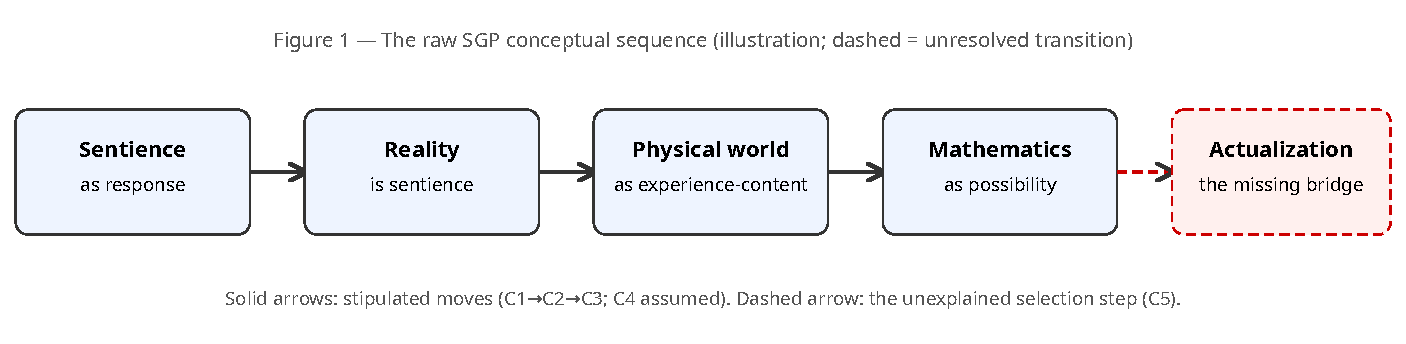
\includegraphics[width=1\linewidth,height=\textheight,keepaspectratio,alt={The raw SGP conceptual sequence (illustration; dashed = unresolved transition)}]{figures/fig1-sequence.pdf}
\caption{The raw SGP conceptual sequence (illustration; dashed =
unresolved transition)}
\end{figure}

\newpage

\chapter{Chapter 4. A World of
Experience-Content}\label{chapter-4.-a-world-of-experience-content}

\textbf{The proposal:} If reality is sentience, what are tables, stars,
and electrons? SGP's answer: they are \emph{experience-content} --- what
sentience contains, not what causes it.

\section{The constitutive claim}\label{the-constitutive-claim}

The third commitment {[}SGP-commitment{]}:

\begin{quote}
``The physical universe is experience-content (a constitutive claim:
physical objects are what sentience contains, not what sentience is
caused by).'' (RESEARCH\_DIRECTOR\_STRATEGIC\_REORIENTATION.md:347)
\end{quote}

Earlier record-language: ``the `world' as experienced,'' ``experienced
manifestation of stable mathematical organization'' (see research-map
03-terminology-map). Note the dependency the reviews later exposed: this
claim depends on the first two commitments \emph{and} on actualization
(C3 depends on C5 --- RD-002) --- because ``content'' that never
stabilizes into anything persistent is not a world at all.

\section{An illustration (not
evidence)}\label{an-illustration-not-evidence}

\emph{{[}Author-inference --- illustration.{]}} Consider a dream. While
dreaming, mountains, people, and weather appear --- vivid, structured,
consequential within the dream. Nothing in the dream is \emph{caused by}
physical mountains; the mountains are \emph{contents of} the dreaming.
SGP proposes, as a philosophical interpretation, that waking physical
reality stands to fundamental sentience the way dream-mountains stand to
the dreamer: contained, not causing.

The analogy breaks where all analogies break: dreams are private,
unstable, and lawless in ways physics is not. SGP's entire research
program is the attempt to close that gap --- to explain stability,
shareability, and mathematical lawfulness from the starting point. The
analogy motivates the question; it answers nothing.

\section{What this changes, and what it leaves
unexplained}\label{what-this-changes-and-what-it-leaves-unexplained}

It changes the \emph{direction of explanation}: instead of asking how
objects generate experience, you ask how experience generates (stable,
shared) objects. It reframes persistence --- ``what survives repeated
interaction'' (glossary:129--130) --- as the central notion, rather than
substance.

It leaves unexplained: \emph{why} any content is stable at all;
\emph{why} different sentient perspectives encounter the \emph{same}
content (the sharing problem); and \emph{why} the stable content is
mathematical. Each ``why'' became a research thread. Stability became
the closure program (Chapters 9--10). Sharing became the composition
investigations (Chapter 12). Mathematicality became the physical-bridge
program (Chapter 13). All three threads end in the same place --- which
is why this book exists.

\section{A word the book will not
use}\label{a-word-the-book-will-not-use}

The records never call ordinary objects ``illusions,'' and neither will
this book. Experience-content can be fully real \emph{as content} ---
the dream-mountain is really in the dream. The claim is about what is
fundamental, not about what is fake. Readers who hear ``unreal'' should
re-read the stipulation: containment is not dismissal.

\section{Where this chapter leaves
you}\label{where-this-chapter-leaves-you-3}

We now have sentience, reality-as-sentience, and a world made of
experience-content. The missing piece is mathematics: why should any of
this be mathematically describable? Chapter 5 introduces possibility ---
and the hardest question of all.

\newpage

\chapter{Chapter 5. The Mathematical Possibility
Problem}\label{chapter-5.-the-mathematical-possibility-problem}

\textbf{The question:} Mathematics is full of structures that
\emph{could} exist. Why does our experience match \emph{these}
structures and not others?

\section{Mathematics as possibility}\label{mathematics-as-possibility}

The fourth commitment {[}SGP-commitment{]}:

\begin{quote}
``Mathematics describes possible structures (a modal claim: mathematics
is about what \emph{could} be, not what \emph{is}).''
(RESEARCH\_DIRECTOR\_STRATEGIC\_REORIENTATION.md:348)
\end{quote}

The reviews call this the least controversial commitment --- ``standard
modal-platonist'' (RD-002) --- and they are right. Consider ordinary
examples {[}Established{]}:

\begin{itemize}
\tightlist
\item
  \textbf{Geometries.} Euclid's parallel postulate can be denied
  consistently. Spherical geometry (no parallels), hyperbolic geometry
  (infinitely many) --- each a complete, consistent world of shapes.
  Mathematics offers all of them. Our local space matches one.
\item
  \textbf{Graphs and relations.} For any finite set of dots, mathematics
  lists \emph{every} possible pattern of arrows between them ---
  2\^{}(n²) patterns for n dots (you will meet this census in Chapter
  7). All are ``possible.'' Almost none describe anything you have seen
  today.
\item
  \textbf{Algebraic structures.} Groups, rings, fields --- infinite
  families, most with no physical application anyone knows.
\end{itemize}

Mathematics is a catalog of could-be. Physics uses a tiny, eerily
effective selection from the catalog. The SGP question: \emph{why this
selection?}

\section{Why possibility alone explains
nothing}\label{why-possibility-alone-explains-nothing}

Here is the trap, stated plainly because the whole book turns on it:
pointing at a structure in the catalog and saying ``reality matches this
one'' is not an explanation. It is a \emph{match}. An explanation needs
the \emph{selector} --- what picked this page of the catalog --- or a
proof that only this page \emph{could} be picked. Without one, you have
correspondence without mechanism: a striking fact, and no account of it.

The Institute understood this. Its fifth commitment names the missing
piece.

\section{Where this chapter leaves
you}\label{where-this-chapter-leaves-you-4}

Possibility is cheap; actuality is the puzzle. Chapter 6 states the
central explanatory challenge --- actualization --- that the entire
mathematical ladder was built to attack.

\newpage

\chapter{Chapter 6. The Missing Bridge:
Actualization}\label{chapter-6.-the-missing-bridge-actualization}

\textbf{The challenge:} A possible structure is not a realized world.
What \emph{actualizes} some possibilities --- and why is there no
mechanism in the records that does it without begging the question?

\section{Possible vs.~realized}\label{possible-vs.-realized}

The fifth commitment {[}SGP-commitment{]}:

\begin{quote}
``Some possibilities become actual (an actualization claim: the
transition from possibility to actuality is the fundamental process).''
(RESEARCH\_DIRECTOR\_STRATEGIC\_REORIENTATION.md:349)
\end{quote}

A weather forecast lists possible storms; one arrives. A die has six
possible faces; one lands up. A mathematical catalog has 2\^{}(n²)
relations on n dots; some pattern is the one your world exhibits. In
each case, \emph{something} narrows could-be to is. Call that something
the actualizer. SGP's ambition --- its ``explanatory ambition'' in
review language --- was to \emph{be} that account: to explain
actualization without smuggling in a new physical force or fitted
parameters.

\section{Why selection cannot simply be
assumed}\label{why-selection-cannot-simply-be-assumed}

Here is the circularity the program had to avoid, and the reader must
see clearly: if your job is to \emph{explain} which possibilities become
actual, you may not \emph{assume} a mechanism that picks them --- unless
you then explain the mechanism. A selector that is just postulated is
the mystery restated, not solved. (``The stable structures persist
because a selector selects them'' explains nothing until the selector is
derived from something more basic.)

The records show the Institute wrestling with exactly this. A late
strategic note concedes the problem may be miscast: ``Becoming actual
may not be a selection problem at all'' but a metaphysical question
about possibility and actuality (RD-001:159--160). The frozen verdict is
sterner: ``actualization without selection is\ldots{} entirely standard
mathematics (differentiator + instability)'' --- a mathematical truism,
not an SGP discovery (RD-002:127, citing Exp21:445). And the selector
search itself ended UNRESOLVED (selector audit :83).

\section{The three gaps inside one
bridge}\label{the-three-gaps-inside-one-bridge}

Actualization, as the program learned, is really three sub-questions:

\begin{enumerate}
\def\labelenumi{\arabic{enumi}.}
\tightlist
\item
  \textbf{Differentiation} --- what makes \emph{this} possibility the
  one that happens (rather than nothing happening)? The records' answer:
  a differentiator plus instability suffices, and that is generic
  mathematics (Exp21:174).
\item
  \textbf{Selection} --- what favors \emph{some} possibilities over
  others? Answer: unresolved. Chirality amplifies but does not select
  (Exp20:510); viability dynamics was never validated (7/7 kill tests
  unresolved).
\item
  \textbf{Persistence} --- what keeps the actualized structure stable
  afterward? Answer: partially --- closure mathematics describes
  \emph{what} persists (Part II), but not \emph{why} this rather than
  that persists.
\end{enumerate}

\section{Where this chapter leaves
you}\label{where-this-chapter-leaves-you-5}

The foundation is now fully on the table: sentience (ambiguous), reality
(stipulated), experience-content (constitutive), possibility (catalog),
actualization (missing bridge). The Institute's response was to build a
ladder: derive mathematical structure from response, step by step, and
see if actualization emerges. Part II climbs that ladder --- starting,
in Chapter 7, with the question of whether ``response'' is mathematics
at all.

\newpage

\begin{figure}
\centering
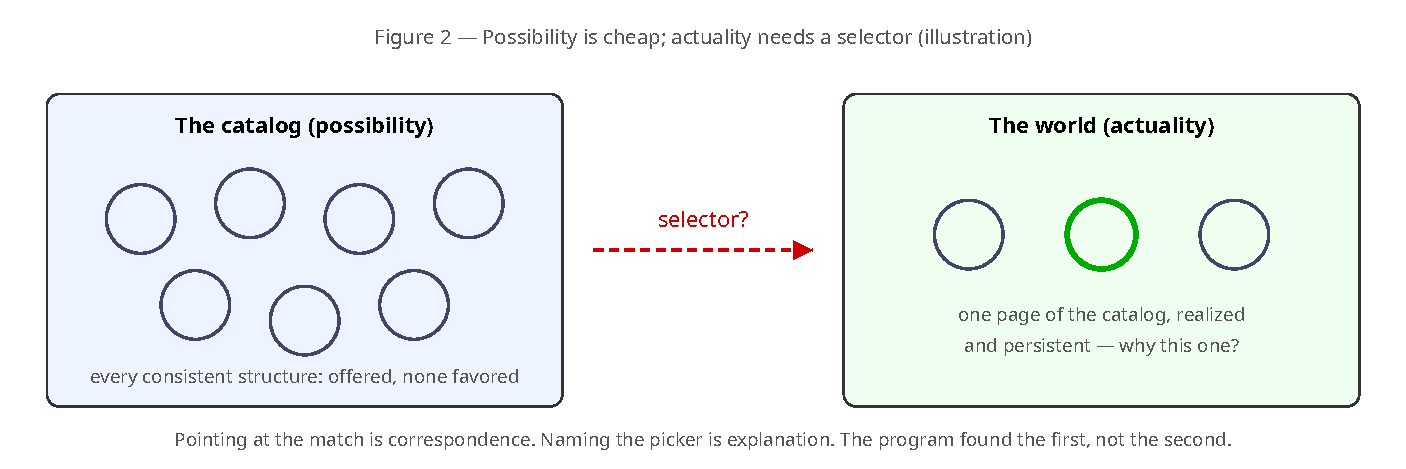
\includegraphics[width=1\linewidth,height=\textheight,keepaspectratio,alt={Possibility is cheap; actuality needs a selector (illustration)}]{figures/fig2-possibility-actualization.pdf}
\caption{Possibility is cheap; actuality needs a selector
(illustration)}
\end{figure}

\newpage

\chapter{Chapter 7. Can Response Become
Mathematics?}\label{chapter-7.-can-response-become-mathematics}

\textbf{The concrete question:} If sentience is ``the ability to
respond,'' does the word \emph{response} add any mathematics beyond an
ordinary \emph{relation}? The Institute tested this by brute force ---
every relation on every set of size up to four --- and got a clean
answer.

\section{What ``response'' was taken to
mean}\label{what-response-was-taken-to-mean}

The tested operationalization {[}SGP-commitment --- the functional
reading{]}: a response is the existence of at least one connection.
Formally: given a finite set X and a relation R (a specification of
which things connect to which --- see below), \texttt{response(R)} holds
exactly when R is nonempty (Exp24:59--63).

What is a relation, plainly? Take a set of dots, say \{0, 1, 2\}. A
(binary) relation is a list of arrows between dots --- including arrows
from a dot to itself. ``0 connects to 1'' is the ordered pair (0,1).
Every possible list is a relation; the empty list is the empty relation.
That is all.

\section{The census: 66,067 records}\label{the-census-66067-records}

How many relations exist on small sets? On n dots there are n² possible
arrows, each present or absent: 2\^{}(n²) relations. For n = 0, 1, 2, 3,
4 that gives 1 + 2 + 16 + 512 + 65,536 = \textbf{66,067} records
{[}Author-inference --- checkable arithmetic{]}. (Some records say
66,066: that count excludes the empty carrier. Same census, stated both
ways; the book uses 66,067 for the total and notes the convention.)

The audit (Experiment 24, 2026-10-08) checked the response predicate
against all 66,067 --- engine 29/29 parts green, deterministic rerun ---
plus 8 richer formalisms (function graphs, causal models, information
channels, dynamical sequences, and more), 10 killer counterexamples, 15
candidate distinguishing properties, and 7 literature controls (Exp24
header; :59--63).

\section{The result}\label{the-result}

\texttt{response(R)\ ⟺\ R\ ≠\ ∅} held for \textbf{all 66,067 relations
--- 0 violations} (Exp24:61, 319, 363) {[}Finite-check{]}. Of the 15
candidate properties that might have separated an SGP-response from a
bare relation, the required count was \textbf{0} (:96). The four-way
classification came out A=1, B=15, C=0, D=0 (:272, :408). The kill
criterion fired under all 8 formalisms (:363). Final verdict (:412)
{[}Negative{]}:

\begin{quote}
RESPONSE REDUCES TO ORDINARY RELATIONAL MATHEMATICS.
\end{quote}

Zero formal novelty ``at this level'' (:69).

\section{What this means --- and what it
doesn't}\label{what-this-means-and-what-it-doesnt}

What it means: under the tested formulation, ``response'' is the word
\emph{nonempty} applied to a relation. The word does interpretive work
(it tells you how to \emph{read} the mathematics --- as responding
rather than merely connecting), but it does zero mathematical work.
Anyone who hoped the foundation conceals a new formal property now knows
exactly where it doesn't.

What it doesn't mean: it does not refute the stipulation (Chapter 3) ---
stipulations aren't refutable. It does not touch the phenomenal
``capacity to feel'' reading, which was never operationalized. It does
not settle every philosophical meaning of response --- only the tested
one. And finite scope (\textbar X\textbar{} ≤ 4) is a limitation to
state, not hide: the claim is ``no distinction in 66,067 cases,'' not
``no distinction anywhere.'' (Though the follow-up formalisms, which are
not size-bound, point the same way.)

\section{Where this chapter leaves
you}\label{where-this-chapter-leaves-you-6}

Response, as tested, is an ordinary relation with an evocative name. But
relations have internal structure --- direction, self-connection,
iteration --- and the program next asked whether \emph{that} structure
yields anything distinctive. Chapter 8 takes relations apart.

\newpage

\chapter{Chapter 8. Direction, Identity, and
Connection}\label{chapter-8.-direction-identity-and-connection}

\textbf{The question:} Relations have direction (arrows point),
self-connection (loops), and multiplicity (many arrows). Are any of
these \emph{SGP's} discovery --- or just ordinary relation theory?

\section{Why direction matters (and what it
is)}\label{why-direction-matters-and-what-it-is}

An ordered pair (x, y) is not the same as (y, x): the arrow points from
x to y. The audit of minimal response mathematics found that this
\emph{orientation} is forced --- it comes free with ordered pairs ---
while two stronger properties are optional {[}Math-verified-as-audit{]}:

\begin{itemize}
\tightlist
\item
  \textbf{Reciprocity} (x→y implies y→x): OPTIONAL. One-way streets
  exist.
\item
  \textbf{Asymmetry} (x→y forbids y→x): OPTIONAL. Two-way streets exist.
\item
  \textbf{Self-response} (x→x, a loop): a separate, independent option.
\end{itemize}

So direction is unavoidable, but it does not smuggle in causation,
influence, or information. Source and target are \emph{tuple slots}, not
agents and patients. This is the first unavoidable mathematical content
of the program --- and it is also the most borrowed: every database
join, every directed graph, every order relation already works this way
{[}Established{]}.

\section{The readings the program could not
separate}\label{the-readings-the-program-could-not-separate}

Three natural strengthenings of ``response'' were tested --- call them
readings B, C, D (roughly: bare connection, structured interaction,
causally-loaded response). Result: all three are COMPATIBLE with the
mathematics, and SGP does not distinguish them
(SGP\_MINIMAL\_RESPONSE\_MATHEMATICS\_09.md:39--46, 51--56). Whatever
separates a mere connection from a genuine interaction, it is not in the
ordered pairs.

\section{Multiplicity and iteration}\label{multiplicity-and-iteration}

Arrows can repeat, chain, and cycle: x→y→z→x. Chaining gives
\emph{reachability} (who can eventually reach whom) --- the seed of the
closure program in Chapter 9. Nothing here is SGP-specific either;
reachability is graph theory's oldest idea. The reader should feel the
pattern forming: each rung finds real structure that turns out to be
standard.

\section{The lesson: discovery
vs.~ownership}\label{the-lesson-discovery-vs.-ownership}

This chapter's moral is the book's recurring discipline: discovering a
\emph{useful distinction} (direction matters!) is not discovering a
distinction \emph{uniquely implied by SGP}. Orientation is worth having
in the toolkit. It just isn't evidence for the framework. Confusing the
two --- ``we use direction, direction is fruitful, therefore our
foundation is fruitful'' --- is the exact slide the audits were built to
catch.

\section{Where this chapter leaves
you}\label{where-this-chapter-leaves-you-7}

Bare relations and their directions are standard. But relations
\emph{do} something: they generate consequences --- everything
reachable, everything implied. Different relations can generate the
\emph{same} consequences. Classifying that phenomenon is the program's
first genuine mathematical contribution. Chapter 9 begins with closure.

\newpage

\chapter{Chapter 9. When Different Connections Produce the Same
Result}\label{chapter-9.-when-different-connections-produce-the-same-result}

\textbf{The intuitive idea:} Two road networks can serve the same
cities. Two different wirings can light the same rooms. Two different
relations can have the same \emph{consequences} --- and the family of
relations sharing consequences can be mapped completely. That map is the
Institute's strongest mathematical work.

\section{Closure in plain language}\label{closure-in-plain-language}

Fix a set S (dots) and a relation R (arrows). A subset A is
\emph{invariant} if no arrow leads out of it: R(A) ⊆ A --- everyone you
can reach from inside A is still inside A. The collection of all
invariant subsets, Inv(R), is the relation's \emph{consequence
structure}: what stays put under the connections.

Two relations with the same invariant family are, for this purpose,
interchangeable. The \emph{fiber} over a consequence-structure C is the
set F\_C = \{R : Inv(R) = C\} --- all wirings with the same
consequences. The program's question: what does a fiber look like?

\section{The closure program: what was
established}\label{the-closure-program-what-was-established}

Working through dozens of numbered results (R19--R51; full index in
Appendix D), the program established {[}Math-verified{]}:

\begin{itemize}
\tightlist
\item
  \textbf{Minimality (R29, corrected R30).} The invariant family is the
  \emph{least} closure system consistent with the relation --- the
  smallest consequence-structure containing everything the arrows force.
\item
  \textbf{Collapse (R31).} Three descriptions --- invariant subsets,
  closure system, closure operator --- are one canonical object viewed
  three ways.
\item
  \textbf{Universality (R40).} The construction works for \emph{any}
  relation on \emph{any} set, as a left adjoint (inclusion-reversing:
  the functor is contravariant, a correction the audits caught and
  kept).
\end{itemize}

And it falsified, cleanly {[}Negative{]}:

\begin{itemize}
\tightlist
\item
  \textbf{Reconstruction is FALSE (R35).} The hope: consequences
  determine wiring (up to renaming). The counterexample at
  \textbar S\textbar=3: f1 = \{0↦1, 1↦0, 2↦1\} and f2 = \{0↦1, 1↦0,
  2↦0\} share I\_f = \{∅, \{0,1\}, S\} but differ --- the stray
  transient points at different partners. (26 such pairs at
  \textbar S\textbar=4.) Root cause: minimal invariant sets are
  \emph{cycles}, not singletons. Consequences forget transients;
  dynamics remembers them. This is a real theorem-shaped hole: closure
  cannot see everything.
\item
  \textbf{Convex sublattices FALSE (R46.1 → R50).} The conjecture that
  fibers are nicely convex sublattices died on 7 counterexamples at
  \textbar S\textbar=3 (intersection of relations can break the
  invariant family: Inv(R1∩R2) ⊋ Inv(R1)∩Inv(R2)).
\end{itemize}

\section{The repair: what fibers actually
are}\label{the-repair-what-fibers-actually-are}

The maximum survived where the minimum didn't. A formula once claimed to
give the \emph{minimal} wiring (R44) actually gives the \textbf{unique
MAXIMUM} R\_C of the fiber (R45 correction; at \textbar S\textbar=3, 13
of 29 systems expose the error). And the fiber itself is a
\textbf{finite poset with a unique maximum} --- ordered by inclusion,
topped by R\_C, but not closed under union/intersection, not convex, not
a lattice (R51 repair).

\section{The manuscript: Fibers of the Relation-to-Closure
Correspondence}\label{the-manuscript-fibers-of-the-relation-to-closure-correspondence}

This became a paper (submission text at
papers/paper3\_kernel\_geometry/final/paper3\_submission.tex; the
top-level paper.tex does not exist in this tree). Its abstract, verified
against the source, claims: Φ: Rel(S) → ClSys(S) sends each relation to
its invariant family; the image is exactly the Alexandrov topologies
containing ∅; every fiber has a unique maximal element R\_C; edges of
R\_C split into essential vs.~conditionally removable; fibers are finite
posets with unique maximum; the convex-sublattice conjecture is false;
results hold for arbitrary sets and relations.

The manuscript's internal record adds: exhaustive checks at
\textbar S\textbar≤4 (29 closure systems at n=3, 355 at n=4 --- later
refined to T0 counts 19/219; Chapter 11), an adversarial verification
pass (R64), a literature-attack pass (R65) behind the novelty sentence
(``the internal order structure of the fibers\ldots{} has not previously
been investigated'' --- with an internal caveat that the material is
elementary and could be folklore), and a completed release checklist
with compiled PDF.

\textbf{Book stance, stated plainly:} the theorems are reported as
\emph{manuscript claims} with stated proofs and finite checks plus
internal hostile audits. Independent verification --- peer review ---
remains. The book does not declare the paper correct, novel, or
publishable. (Appendix D indexes every theorem; Appendix K lists the
verification scope.)

\section{Why this rung matters}\label{why-this-rung-matters}

This is the only rung that produced candidate new mathematics rather
than a boundary result --- and even here, the content belongs to order
theory and topology, not to sentience. The fiber theorems never mention
response, experience, or SGP. That independence is both the rung's
strength (the math stands alone) and the program's problem (the math
doesn't need the philosophy). Chapter 10 follows the one specialization
that gave back a closed-form answer.

\newpage

\begin{figure}
\centering
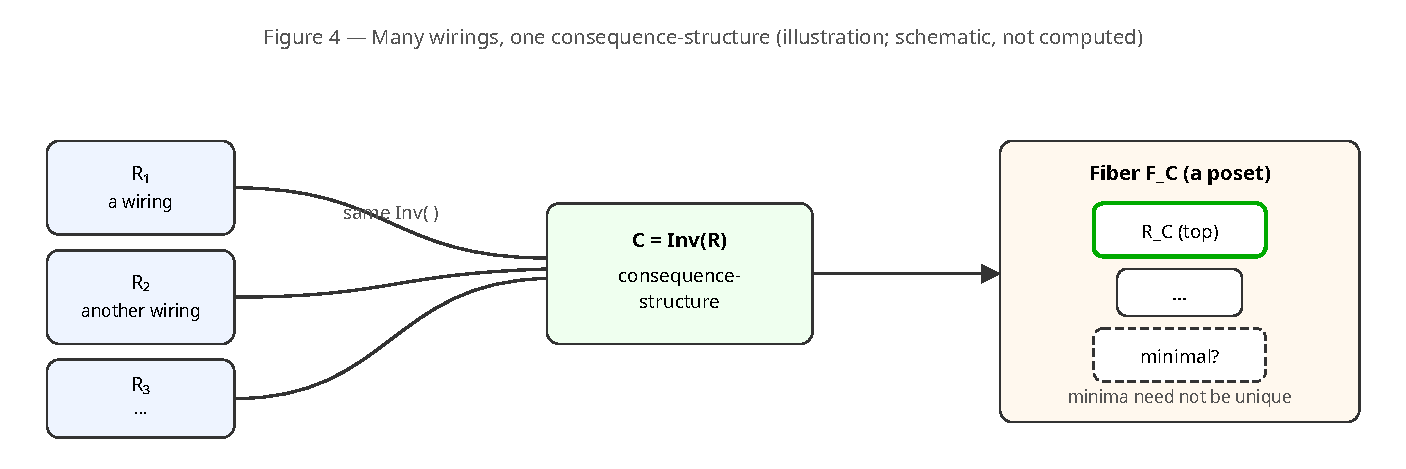
\includegraphics[width=1\linewidth,height=\textheight,keepaspectratio,alt={Many wirings, one consequence-structure (illustration; schematic)}]{figures/fig4-relation-closure.pdf}
\caption{Many wirings, one consequence-structure (illustration;
schematic)}
\end{figure}

\newpage

\chapter{Chapter 10. The Geometry of
Consequences}\label{chapter-10.-the-geometry-of-consequences}

\textbf{The puzzle:} Chapter 9 mapped fibers in general but left one
question open: \emph{how many} wirings share a given
consequence-structure? For the special case of orderings ---
prerequisite chains, task hierarchies --- the answer turns out to be
exact.

\section{Partial orders and lower sets,
plainly}\label{partial-orders-and-lower-sets-plainly}

A \emph{partial order} is a ranking where some pairs compare and others
don't: prerequisites (``learn fractions before algebra''), task
dependencies, or simply 0 \textless{} 1 \textless{} 2 with gaps. A
\emph{lower set} is a collection closed downward: if a task is included,
so are all its prerequisites. The lower sets of a poset form a closure
system --- our consequence-structure from Chapter 9, in ordered
clothing.

\section{The manuscript's answer}\label{the-manuscripts-answer}

The second manuscript (\emph{Relations Inducing a Finite Poset's
Lower-Set Closure}, papers/paper4\_fiber\_complexity/paper\_v3.tex ---
verified against the source) proves {[}Math-verified-as-manuscript{]}:

\begin{quote}
\textbf{Theorem.} For a finite partial order (S, ≤), the inducing
relations form a fiber F in canonical bijection with P(S) × P(E): φ(A,
E′) = \{self-loops on A\} ∪ T ∪ E′. Hence \textbar F\textbar{} =
2\^{}\textbar S\textbar+\textbar E\textbar.
\end{quote}

In words: every wiring with these consequences consists of three
independent choices --- which dots get self-loops (any subset A); the
\emph{covering} pairs T (mandatory: each prerequisite link with nothing
between must be wired directly, since no detour exists); and any subset
E′ of the \emph{non-covering} comparable pairs E (optional shortcuts ---
a direct wire paralleling a chain changes nothing reachable).

The proof is four short paragraphs (verified in the source): loops never
affect reachability; every inducing wire must run downhill (contained in
R\_≤); shortcut subsets preserve consequences via covering chains;
covering pairs are unavoidable. Worked instances: a 3-chain gives
\textbar F\textbar{} = 16; a 4-chain 128; a pure antichain 2\^{}n; a
V-shape (a\textless c, b\textless c) gives 8. The manuscript reports
exhaustive checks over all finite partial orders on up to 5 elements (1,
3, 19, 219, 4231 --- the standard labeled-poset counts) with zero
violations {[}Finite-check{]}. (One provenance detail worth preserving:
version 3 corrects version 2's abstract --- ``covering'' to
\emph{non-covering} comparable pairs. The records correct themselves;
the book keeps the correction visible.)

\section{New rung or same rung?}\label{new-rung-or-same-rung}

A genuine specialization that answers a question the general theory left
open (the count). The abstract edge-classes of Chapter 9 --- essential
vs.~conditionally removable --- become concrete here: covering
vs.~non-covering pairs. The ladder grows by \emph{specification}, not by
new foundations. Same verdict as before, sharpened: beautiful order
theory; no sentience in it.

\section{Where this chapter leaves
you}\label{where-this-chapter-leaves-you-8}

We can now count wirings exactly --- for ordered consequences. But a
crack appeared in the general picture: the product decomposition fails
for some consequence-structures. The failure has a name (non-T0), a
precise location (one lemma), and a complete classification. Chapter 11
is about what representations preserve --- and what they silently drop.

\newpage

\chapter{Chapter 11. What a Mathematical Representation
Preserves}\label{chapter-11.-what-a-mathematical-representation-preserves}

\textbf{The question:} When you describe two structures separately, then
combine them, do you still know what you have? Sometimes the combination
step silently discards the one piece of information that mattered.

\section{The T0 surprise}\label{the-t0-surprise}

The fiber product decomposition (Chapters 9--10) broke on 10 cases at
\textbar S\textbar=3 --- and \emph{all 10} shared one property: non-T0.
(T0, plainly: the consequence-structure distinguishes every pair of dots
--- no two dots sit in exactly the same invariant sets. Posets always
qualify; that is why Chapter 10 never saw the problem.) At
\textbar S\textbar=4: zero violations among all 219 T0 systems
{[}Finite-check{]}. T0 is not a technicality; it is the \emph{exact
boundary}: the paper's abstract and theorems were corrected to include
it (R88/R89 records).

The audit traced the first failure to a single lemma --- the Path Lemma
(Lemma 3.3): it holds for all T0 systems tested and fails for all non-T0
ones. And the non-T0 fibers were completely classified: self-loop
choices times strongly-connected digraphs --- structured, but not
Boolean (verified 10/10). No natural generalization exists. This is the
program's cleanest boundary result: a hypothesis shown \emph{necessary},
not merely sufficient, with the failure mechanism named.

\section{The composition boundary
(C3)}\label{the-composition-boundary-c3}

A second representation result, equally sharp: if you classify two
relations \emph{separately} (their isomorphism classes) and then compose
them, you cannot in general determine the composite's class --- the
\emph{alignment} of the shared middle set is lost. Joint classification
determines composition; separate classification does not (for
\textbar S\textbar{} ≥ 2; the boundary sits exactly at
\textbar S\textbar{} = 1). The lost information has a name:
shared-carrier alignment.

Why does this matter to SGP? It was attacked as a possible source of
novelty --- perhaps ``interaction'' lives in the alignment that separate
descriptions drop. The audit's answer: the boundary theorem is standard
equivariance mathematics. Genuine, useful, and not SGP-specific
{[}Negative on novelty; Math-verified on content{]}. It also did not
move the Interaction priority score (see Chapter 12).

\section{The moral: representation is
load-bearing}\label{the-moral-representation-is-load-bearing}

Two lessons the book carries forward. First, what survives a change of
representation is the real content --- and both results pass that test
(they are representation-invariant theorems \emph{about}
representation). Second, the program kept hoping that the \emph{gap}
between a structure and its description would contain new mathematics.
It contains real mathematics, but known mathematics. The gap is a
workplace, not a goldmine.

\section{Where this chapter leaves
you}\label{where-this-chapter-leaves-you-9}

Structure, order, boundaries: the program's mathematics is solid and
standard. The promised land was always one rung higher ---
\emph{interaction} and \emph{selection}, where dynamics would favor some
structures over others. Chapter 12 climbs there, and finds the ladder
leaning against nothing.

\newpage

\chapter{Chapter 12. Can Interaction Explain Anything
New?}\label{chapter-12.-can-interaction-explain-anything-new}

\textbf{The temptation:} Surely \emph{interaction} --- things affecting
each other, composing, competing, persisting --- must add something
beyond frozen relations. The Institute attacked this hope eleven times.
Every attack ended the same way.

\section{The audit that closed the
question}\label{the-audit-that-closed-the-question}

The Compass I boundary audit reviewed every prior assault on the
Interaction debt --- the interaction-primitive program, the
response-first deep audit, the invariance audit, Exp24, Exp25, the C3
results, Road D, Stage 1 --- plus the standard comparison frameworks,
and tested six candidate distinctions between ``arbitrary relation'' and
``interaction system.'' Classification: NO QUALIFYING MATHEMATICAL
QUESTION FOUND. Three of seven stop conditions fired: all candidates
answered by established mathematics; novelty evaporating under standard
terminology; every result a restatement, routine corollary, or
reclassification.

The audit's honest sentence deserves quoting in full {[}Negative{]}: the
Interaction debt ``is not blocked by a missing question. It is blocked
by the fact that the questions that can be precisely stated about
interaction have already been answered by existing mathematics --- and
the questions that cannot be precisely stated without SGP-specific
primitives are not mathematical questions at all.''

Ordinary mathematics already represents interaction richly ---
relations, morphisms, composition, dynamical systems, process theories.
The program kept offering new words for these; the audits kept
translating them back.

\section{Selection: amplification is not
choice}\label{selection-amplification-is-not-choice}

Three experiments form the selection triptych {[}Negative{]}:

\begin{itemize}
\tightlist
\item
  \textbf{Exp20 (chirality):} symmetric dynamics can \emph{amplify} an
  initial asymmetry --- but amplification is not selection. Starting
  exactly symmetric stays symmetric. A megaphone is not a judge.
\item
  \textbf{Exp21 (actualization):} actualization without a selector is
  generic mathematics --- a differentiator plus instability suffices.
  Something happens rather than nothing for entirely ordinary reasons.
  Actualization is ∃ (existence), not ∃! (unique choice).
\item
  \textbf{Exp19 (plurality):} multiple internally coherent models
  coexisting is generic mathematics with zero SGP residue. Plurality is
  the default; convergence needs explaining, not divergence.
\end{itemize}

And the positive searches failed: the selector's source is UNRESOLVED
(selector audit :83); viability dynamics (coherence + stability +
fertility) was never validated --- all 7 kill tests unresolved;
composition of sentient processes turned out generic (non-sentient
processes do the same --- SAO-1). A late proposal (shared perspectives →
generality → imbalance → selection) broke on four of six links and
recycled familiar philosophy (RD-003; see Chapter 20).

\section{What ``no'' means here}\label{what-no-means-here}

Not ``interaction is meaningless'' --- the audit explicitly refuses that
reading. It means: the \emph{tested attempt} to derive distinctive
mathematics from interaction yielded standard mathematics. Interaction
remains real, rich, and studied --- by the ordinary sciences of
dynamics, which need no SGP primitive.

\section{Where this chapter leaves
you}\label{where-this-chapter-leaves-you-10}

mathematics could not deliver the bridge, perhaps \emph{physics} could:
even standard mathematics might constrain which physical structures are
possible. Chapter 13 tests that hope --- with the program's strictest
gates.

\newpage

\chapter{Chapter 13. From Mathematics to
Physics}\label{chapter-13.-from-mathematics-to-physics}

\textbf{The hope:} Even if the abstract mathematics is standard, perhaps
SGP \emph{constrains physics} --- ruling out some physical structures,
requiring others, predicting something new. Three investigations tested
this, with pre-registered gates. All three closed negative.

\section{The grammar test: C1--C4 exclude
nothing}\label{the-grammar-test-c1c4-exclude-nothing}

Stage 1 asked whether the program's four grammar items (relation
iteration, relational hierarchy, composition, term rewriting ---
\emph{not} the philosophical C1--C5 of Chapter 2; see the label warning
in Chapter 1) exclude any mathematically possible structure beyond
ordinary relational algebra. Answer: ``PRIOR RESULTS ALREADY SETTLE THE
QUESTION'' --- they define no admissibility predicate; they exclude
nothing structurally (FOUNDATIONAL\_CLARIFICATION\_STAGE1.md:59--69,
193--200) {[}Negative{]}. A grammar that permits everything constrains
nothing.

\section{Exp25: seven domains, zero
distinctions}\label{exp25-seven-domains-zero-distinctions}

The physical-distinction audit ran seven candidate domains (measurement,
entanglement, quantum gravity, renormalization, gauge,
symmetry-breaking, biology) through forks, operationalization criteria,
observer-replacement tests, representation-equivalence pairs, and
engineered predictions. Result: all seven claims Level A (interpretive
correspondence) only; B = 0, C = 0; 0 selections among 7 genuine
unresolved forks {[}Negative{]}. Both success boxes --- ``SGP requires a
structure standard theory permits but does not require'' and ``SGP
predicts an unconfirmed observable'' --- FAIL (verified §25). All eight
kill conditions held, including: every correspondence interpretive-only;
every restriction already ordinary mathematics; every choice supplied by
empirical input; every ``selection'' merely amplification (verified
§26). Final box: ``SGP HAS NOT YET ACQUIRED EMPIRICAL CONTENT'' --- with
the explicit note that this does \emph{not} claim SGP is false; it kills
the empirical \emph{bridge}, leaving the stipulation untouched.

\section{Road D: no qualifying
target}\label{road-d-no-qualifying-target}

The residual-anomaly search screened six pools (neutrino ordering,
strong CP, cosmological constant, dark matter, and others) against seven
gates. 0/6 advanced; every candidate failed D6 --- connecting to physics
required arbitrary encoding or target-specific information the
governance rules forbid {[}Negative{]}.

\section{Interpretation vs.~constraint
vs.~prediction}\label{interpretation-vs.-constraint-vs.-prediction}

The chapter's discipline --- the book's discipline --- is a four-way
split the records enforce:

\begin{itemize}
\tightlist
\item
  An \textbf{interpretation} of physics (a new way to read existing
  theory) --- achieved repeatedly (Level A).
\item
  A \textbf{mathematical restriction} on possible models --- never
  achieved (B = 0).
\item
  A \textbf{new explanatory mechanism} --- never achieved.
\item
  A \textbf{falsifiable prediction differing from alternatives} ---
  never achieved (C = 0).
\end{itemize}

Interpretations are not worthless. But they are not explanations, and
the program's ambition required explanations.

\section{Where this chapter leaves
you}\label{where-this-chapter-leaves-you-11}

The ladder is fully climbed: relations (standard), orientation
(standard), closure (real theorems, standard field), posets (exact
counts, standard field), boundaries (sharp, standard), interaction (no
new question), physics (no new constraint). Chapter 14 steps back and
asks what the climb was \emph{worth}.

\newpage

\chapter{Chapter 14. The Ladder's
Payoff}\label{chapter-14.-the-ladders-payoff}

\textbf{The synthesis question:} After eight rungs, what does the
program actually own --- and what does the gap between ambition and
consequence mean?

\section{What the ladder revealed
(kept)}\label{what-the-ladder-revealed-kept}

Genuine mathematical content, each piece labeled as in the chapters
{[}Math-verified{]} {[}Finite-check{]}:

\begin{enumerate}
\def\labelenumi{\arabic{enumi}.}
\tightlist
\item
  A \textbf{boundary result} on response (Ch. 7): the foundation's
  formal content, measured exactly (0/66,067).
\item
  \textbf{Orientation analysis} (Ch. 8): what ordered pairs force and
  what they don't.
\item
  \textbf{Closure universality and collapse} (Ch. 9): least closure
  systems, three-object unity, contravariant adjunction.
\item
  \textbf{Fiber geometry} (Ch. 9): unique maximum R\_C, edge dichotomy,
  finite-poset fibers, falsified convexity --- in a completed manuscript
  with internal hostile audits.
\item
  \textbf{Poset product decomposition and count} (Ch. 10): P(S)×P(E),
  2\^{}\textbar S\textbar+\textbar E\textbar{} --- in a second
  manuscript, checked to \textbar S\textbar≤5.
\item
  \textbf{Exact boundaries} (Ch. 11): T0 necessity with named failure
  lemma; composition's joint-vs-separate boundary at
  \textbar S\textbar=1 vs ≥2.
\end{enumerate}

All of it belongs to standard mathematics --- order theory, topology,
relation algebra. None of it mentions sentience. That is a fact about
the results, not an insult to them: theorems do not need philosophical
parents to be true.

\section{What the ladder did not
establish}\label{what-the-ladder-did-not-establish}

The distinctive SGP bridge: no new mathematical structure \emph{from}
response (Ch. 7--8), no dynamics \emph{from} closure (R35/R36), no
selector \emph{from} interaction (Ch. 12), no constraint \emph{on}
physics (Ch. 13). The gap between the philosophical ambition (Chapters
1--6) and the derived consequences is now measured, not merely felt.
That measurement \emph{is} the payoff --- for the program's honesty, if
not for its ambition.

\section{Failure vs.~refutation
vs.~boundary}\label{failure-vs.-refutation-vs.-boundary}

Three words the book never interchanges:

\begin{itemize}
\tightlist
\item
  \textbf{Failure} (of an attempt): the bridge program did not reach its
  goal. True, and the program said so itself.
\item
  \textbf{Refutation} (of the foundation): the starting stipulation
  shown false. Never happened --- stipulations can't be refuted, and
  none of the negatives touch the metaphysics.
\item
  \textbf{Boundary} (of a method): the exact edge where a technique
  stops working (T0, \textbar S\textbar=1, Level A). Achieved
  repeatedly, and genuinely valuable: boundaries are what make the next
  attempt smarter.
\end{itemize}

The ladder's story is failure-of-attempt plus boundary-discovery, not
refutation. Readers who want a martyrdom or a triumph will both be
disappointed. What remains is rarer: a complete, documented map of where
an idea stops.

\section{Where this chapter leaves
you}\label{where-this-chapter-leaves-you-12}

Mathematics has spoken: standard tools, honestly audited, no bridge. But
the program also looked outward --- at the famous mysteries of physics
that \emph{seem} to whisper SGP's themes: entanglement, condensation,
identical particles. Part III visits each mystery, explains the real
physics carefully, and asks what it actually implies. The answers may
surprise you --- especially the third.

\newpage

\begin{figure}
\centering
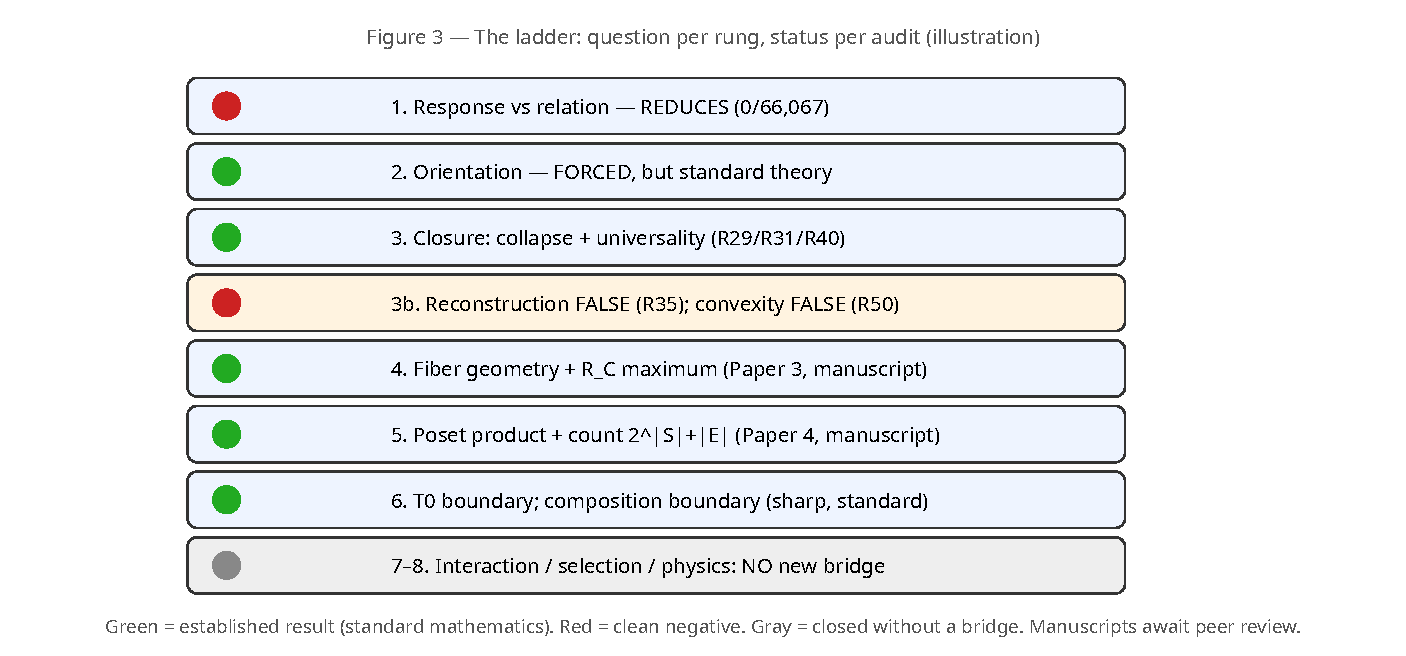
\includegraphics[width=1\linewidth,height=\textheight,keepaspectratio,alt={The ladder: question per rung, status per audit (illustration)}]{figures/fig3-ladder.pdf}
\caption{The ladder: question per rung, status per audit (illustration)}
\end{figure}

\newpage

\chapter{Chapter 15. Entanglement and the Meaning of
Separateness}\label{chapter-15.-entanglement-and-the-meaning-of-separateness}

\textbf{The question everyone asks:} Does quantum entanglement show that
``everything is really one'' --- and does that prove SGP? The physics is
real and astonishing. The inference to SGP is not licensed. This chapter
separates them.

\section{What entanglement is
{[}Established{]}}\label{what-entanglement-is-established}

A quantum state describes a system by a vector (think: an arrow encoding
all measurable tendencies). A \emph{joint} state of two systems,
\textbar Ψ⟩\_AB, can be \emph{entangled}: it cannot be factored into
``state of A times state of B.'' Measure A, and the outcomes correlate
with measurements on B in ways no pre-arranged classical plan can mimic.
The reduced state of A alone --- ρ\_A, obtained by the \emph{partial
trace} over B --- is a projection: a shadow of the whole, not a complete
description of a part.

In 1964 Bell proved the point mathematically: models satisfying locality
plus hidden variables must obey inequalities that quantum statistics
violate (Bell 1964, Physics Physique Fizika 1:195--200). Experiments
confirmed the violation --- Aspect's 1982 tests, and definitively the
2015 loophole-free tests over 1.3 km of electron spins (Hensen et al.,
Nature 526:682--686; S = 2.42 ± 0.20 against the classical bound S ≤ 2).
Local hidden variables are empirically ruled out.

\section{What the correlations do NOT
do}\label{what-the-correlations-do-not-do}

They do not permit controllable faster-than-light communication
{[}Established{]}. This is the no-signaling theorem: the marginal
statistics at B are independent of which measurement was chosen at A.
You can share randomness faster than light could carry it, but you
cannot \emph{send a message} with it. Every ``quantum telephone'' idea
dies on this theorem. (Figure 5 diagrams the setup: correlated outcomes,
crossed-out signal arrow.)

``Nonlocality'' itself means different things in different
interpretations {[}Established{]}: in collapse readings, something
discontinuous happens at measurement; in Everett, there is no collapse
and correlations are branch structure; in Bohm, there is genuine
nonlocal guidance plus unobservable preferred frame. The experiments
constrain models; they do not select an interpretation. Anyone who tells
you Bell tests ``prove'' their favorite metaphysics is selling
something.

\section{What the Institute said --- and what it
found}\label{what-the-institute-said-and-what-it-found}

SGP's interest was the founding pattern ``one mathematical whole →
apparently many spacetime things'': ONE joint state, experienced as two
particles (physics-cases inventory: ``ONE state → two particles.
PASS.''). As interpretation, it fits: entanglement \emph{is} a case of
joint-state priority {[}SGP-interpretation{]}.

But the bridge audits found zero delta {[}Negative{]}:
``beyond\_standard\_adds = {[}{]}\ldots{} No new restriction''
(Exp25:139--141); the GHZ-vs-W entanglement classes are ``ordinary
linear algebra,'' no SGP constraint (Bridge Q1); Bell/CHSH tests are
``standard quantum optics,'' relabeled thresholds, ``falsifiable but not
SFH-testing'' (T700 audits). The physics examples were downgraded by the
Institute itself: 0 evidence, 12 analogy, 10 irrelevant --- ``No analogy
counts as evidence unless the mathematical structure is demonstrably
shared. It is not.''

\section{The verdict on the whisper}\label{the-verdict-on-the-whisper}

Entanglement does not prove universal consciousness, does not prove SGP,
and does not establish that all objects share one mind. It establishes:
joint states, nonfactorizability, Bell violations, no-signaling.
Everything beyond that is interpretation --- including SGP's.
Interpretations are allowed. They are not results.

\section{Where this chapter leaves
you}\label{where-this-chapter-leaves-you-13}

One flagship mystery: real physics, SGP-neutral. The next ---
condensation --- tempted the program differently: not correlation across
distance, but many particles \emph{becoming one state}. Chapter 16.

\newpage

\begin{figure}
\centering
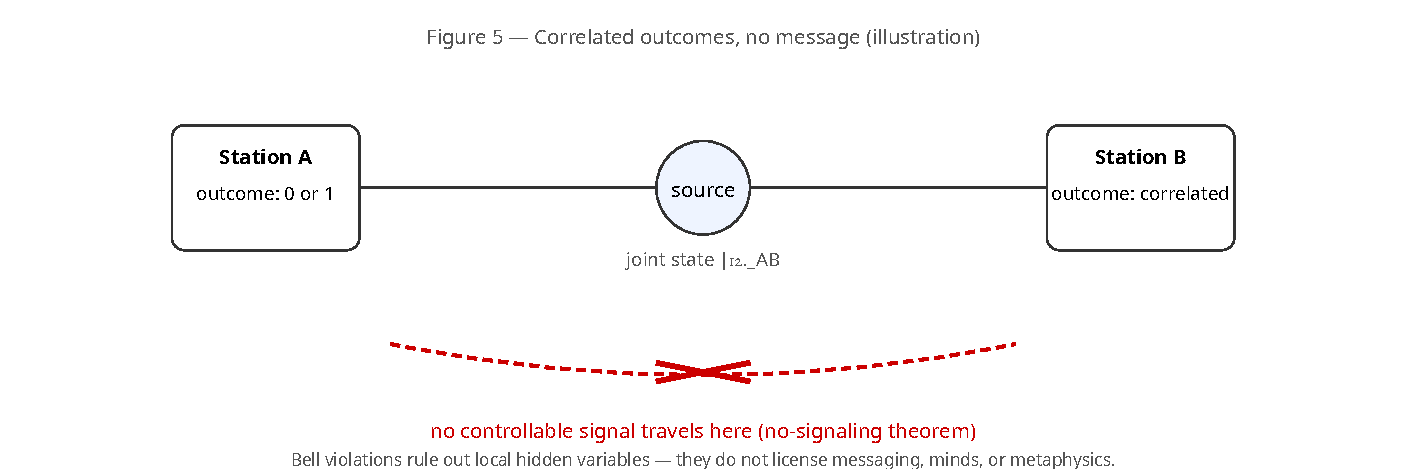
\includegraphics[width=1\linewidth,height=\textheight,keepaspectratio,alt={Correlated outcomes, no message (illustration)}]{figures/fig5-entanglement.pdf}
\caption{Correlated outcomes, no message (illustration)}
\end{figure}

\newpage

\chapter{Chapter 16. Bose--Einstein Condensation and Collective
States}\label{chapter-16.-boseeinstein-condensation-and-collective-states}

\textbf{The image that tempts:} thousands of atoms surrendering
individuality, flowing as one quantum wave. If anything in physics
\emph{looks} like SGP's unity themes, it is BEC. The physics is
gorgeous. The analogy still isn't evidence.

\section{What BEC is {[}Established{]}}\label{what-bec-is-established}

Some particles --- \emph{bosons} (photons, helium-4 atoms, rubidium-87
atoms) --- may share a quantum state without limit, unlike fermions
(electrons), which obey Pauli exclusion. Bose's 1924 counting and
Einstein's 1924--25 extension predicted: cool a dilute boson gas far
enough, and a \emph{macroscopic} fraction piles into the lowest state
--- ``macroscopic occupation of a single quantum state,'' described by
one macroscopic wavefunction φ(x), the order parameter.

In 1995 it was seen: rubidium-87 at \textasciitilde170 nanokelvin
(Anderson et al., Science 269:198--201 --- narrow peak atop the thermal
distribution, abrupt growth on cooling, anisotropic minimum-energy
profile), sodium the same year (Davis et al., PRL 75:3969). The
condensate flows without viscosity, interferes like a single wave, and
is genuinely collective.

\section{What BEC is NOT}\label{what-bec-is-not}

It does not mean all matter becomes one object, or that constituents
lose every distinction {[}Established{]}. Most atoms remain
\emph{outside} the condensate (the thermal cloud); the state is
symmetric under exchange but not Bell-entangled in the
subsystem-correlation sense; position measurements still find atoms
\emph{somewhere}. A condensate is one \emph{mode} massively occupied,
not the universe merging into a blob. (Figure 6 shows the level diagram:
one rung crowded, the rest thinly peopled.)

The Institute's own records make exactly this distinction --- to their
credit: ``IS BEC STRUCTURALLY SAME AS ENTANGLEMENT? YES: one joint
state\ldots{} NO: BEC has macroscopic occupation of one state;
entanglement involves correlations between subsystems. VERDICT: BEC is a
GENUINE case of the pattern. RELATED but DISTINCT''
(sgp\_physics\_cases\_01.py:271--276).

\section{Why BEC attracted the program --- and where it
stopped}\label{why-bec-attracted-the-program-and-where-it-stopped}

Collective organization, common states, large-scale coherence: BEC is
the best physical exhibit for ``many becoming effectively one.'' But the
exhibit never became an argument {[}Negative{]}: all physics-cases
entries stayed Type 1 (genuine structural correspondence) with ZERO
reaching Type 3+ (SGP adds constraint); BEC never even graduated to the
bridge audit's candidate domains; measurement-threshold claims about BEC
coherence were ruled ``falsifiable but not SFH-testing'' --- matching
data confirms standard physics, not SGP (T700.4).

A conceptual analogy motivates a question --- ``could stable shared
structure emerge this way?'' --- but does not answer it. The book's rule
from Chapter 5 holds: similarity is not mechanism.

\section{Where this chapter leaves
you}\label{where-this-chapter-leaves-you-14}

Two mysteries visited, both SGP-neutral. The third --- particle identity
--- is where the mission brief expected an Institute doctrine (``same
particle,'' ``equation-idea''). The records, searched exhaustively,
contain no such doctrine. Chapter 17 reports what they \emph{do}
contain, and why the absence matters more than a discovery would.

\newpage

\begin{figure}
\centering
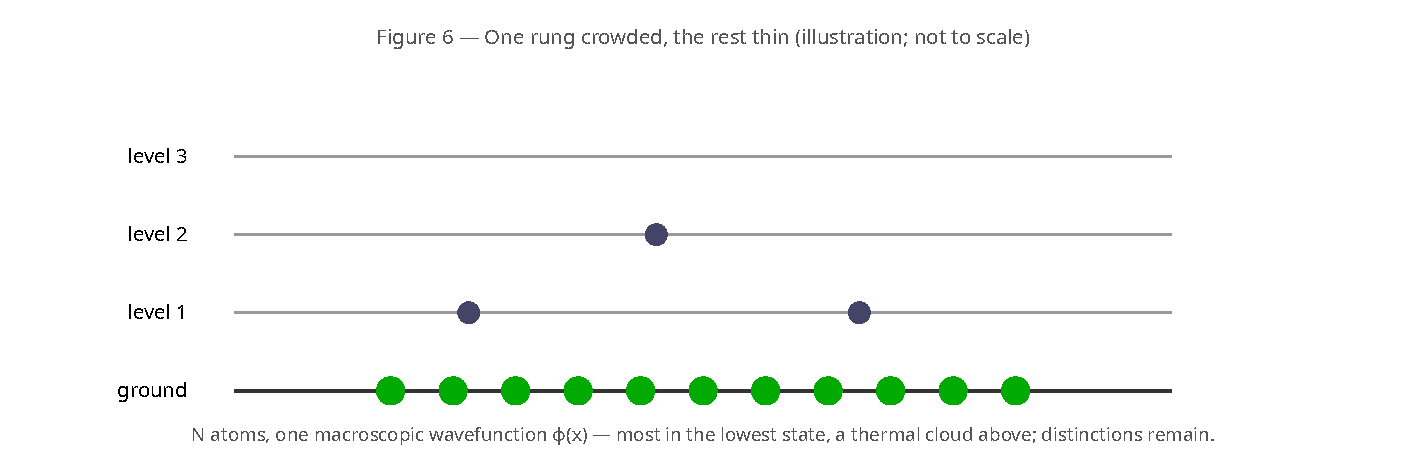
\includegraphics[width=1\linewidth,height=\textheight,keepaspectratio,alt={One rung crowded, the rest thin (illustration; not to scale)}]{figures/fig6-bec.pdf}
\caption{One rung crowded, the rest thin (illustration; not to scale)}
\end{figure}

\newpage

\chapter{Chapter 17. Why Every Electron Is Like Every Other
Electron}\label{chapter-17.-why-every-electron-is-like-every-other-electron}

\textbf{The delicate question:} The mission brief expected an Institute
doctrine here --- a ``same particle'' or ``equation-idea'' formulation,
perhaps claiming electrons and protons are one underlying entity. An
exhaustive search of the records found no such doctrine. This chapter
says exactly what the records contain, explains the standard physics
precisely, and refuses to invent the missing doctrine.

\section{The standard physics, stated exactly
{[}Established{]}}\label{the-standard-physics-stated-exactly-established}

\begin{itemize}
\tightlist
\item
  \textbf{All electrons are identical particles of the same species}:
  same mass, same charge, same spin. Ditto all protons. This is what
  ``identical particles'' means in quantum theory: swapping labels
  changes nothing observable, enforced by symmetrized states (bosons) or
  antisymmetrized states (fermions), organized in Fock space by
  occupation numbers.
\item
  \textbf{Electrons and protons are NOT the same species.} They differ
  in mass (proton ≈ 1836× electron), electric charge (−1 vs +1), spin
  class (electron: elementary spin-1/2 fermion; proton: composite
  spin-1/2 hadron of quarks and gluons), and internal structure
  (electron: pointlike in the Standard Model; proton: bound quark-gluon
  system). (Figure 7 tabulates this.) Identical-particle theory never
  claims otherwise: it identifies particles \emph{within} a species,
  never \emph{across} species.
\end{itemize}

Two different claims must never be merged: (i) every electron is
identical to every other electron --- standard, true; (ii) electrons and
protons are the same underlying entity --- speculative, requiring new
physics and new mathematics, found nowhere in the records.

\section{What the Institute actually
wrote}\label{what-the-institute-actually-wrote}

The records' particle entry reads {[}SGP-interpretation{]}: ``CANDIDATE
2: IDENTICAL PARTICLES --- Object: Symmetrized N-particle state in Fock
space. Represents: single state, no individual particle labels\ldots{}
ONE Fock state → N particles. PASS.'' (sgp\_physics\_cases\_01.py:43,
226). That is claim (i), in standard formalism, with an SGP-style
reading (``no individual labels'' as another instance of
one-whole→many-appearances). Pauli exclusion appears only as ordinary
background (hydrogen shell structure in multi-electron treatments). No
equation unifies electron and proton. No ``same particle'' doctrine
exists: repo-wide searches for ``same particle'' return only null-model
boilerplate; ``equation-idea'' and ``every electron'' return zero hits.

The closest match to ``equation-idea'' is the ONE EQUATION/ONE CONCEPT
HYPOTHESIS (sgp\_physics\_cases\_01.py:219--243): ``Does ONE
mathematical object describe ONE whole, while experience interprets it
as multiple things?'' --- with all 17 candidates passing. Read it
carefully: it is about \emph{formalism} (one equation, many
appearances), not \emph{particle identity}. Conflating the two would
manufacture exactly the doctrine the search failed to find. The book
will not do that.

\section{Why the absence matters}\label{why-the-absence-matters}

A book hunting for SGP's boldest physics claim might be tempted to
upgrade ``no individual labels'' into ``all particles are one entity.''
The records decline the upgrade, and the downgrade audit agrees
(ANALOGY, not evidence). The honest chapter is therefore short: standard
indistinguishability, correctly stated, plus a documented absence where
a legend might have grown. Negative search results are results.

\section{Where this chapter leaves
you}\label{where-this-chapter-leaves-you-15}

The three flagship phenomena are exhausted --- all real, all
SGP-neutral. Remaining: the other frontiers the records touched
(gravity, holography, constants, dark matter) and the question of what
\emph{kind} of contact the program ever made with them. Chapter 18.

\newpage

\begin{figure}
\centering
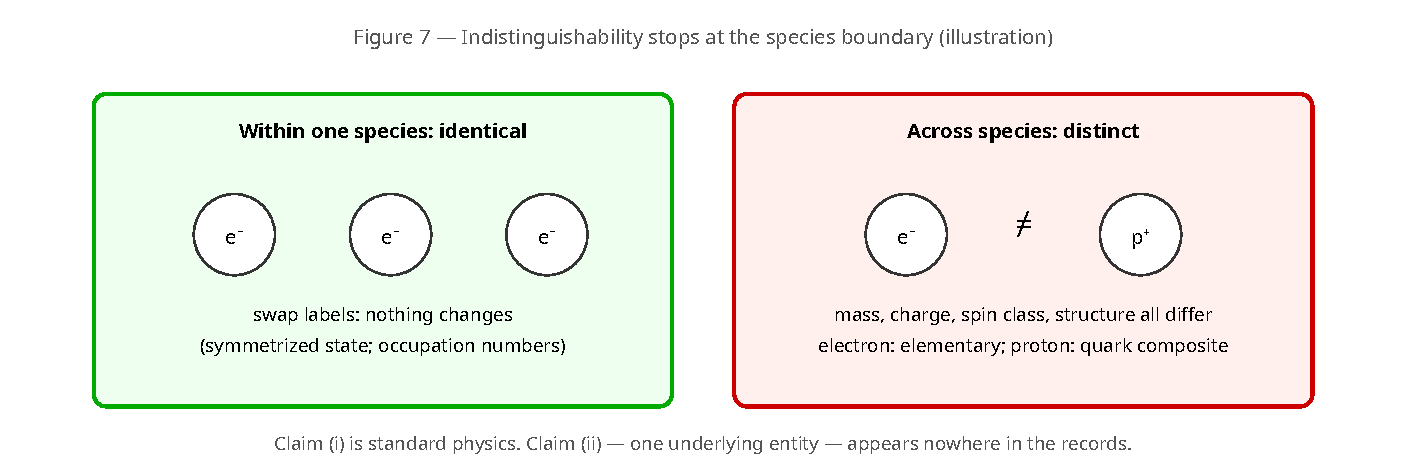
\includegraphics[width=1\linewidth,height=\textheight,keepaspectratio,alt={Indistinguishability stops at the species boundary (illustration)}]{figures/fig7-particles.pdf}
\caption{Indistinguishability stops at the species boundary
(illustration)}
\end{figure}

\newpage

\chapter{Chapter 18. Other Physical
Frontiers}\label{chapter-18.-other-physical-frontiers}

\textbf{The rule for this chapter:} only topics with a \emph{documented}
SGP connection appear. Fame is not a criterion; mystery is not a
criterion. Each entry gets the five-column treatment: phenomenon,
standard account, SGP contact, evidence, status.

\section{Documented contacts (from the
records)}\label{documented-contacts-from-the-records}

\begin{longtable}[]{@{}
  >{\raggedright\arraybackslash}p{(\linewidth - 8\tabcolsep) * \real{0.2000}}
  >{\raggedright\arraybackslash}p{(\linewidth - 8\tabcolsep) * \real{0.2000}}
  >{\raggedright\arraybackslash}p{(\linewidth - 8\tabcolsep) * \real{0.2000}}
  >{\raggedright\arraybackslash}p{(\linewidth - 8\tabcolsep) * \real{0.2000}}
  >{\raggedright\arraybackslash}p{(\linewidth - 8\tabcolsep) * \real{0.2000}}@{}}
\toprule\noalign{}
\begin{minipage}[b]{\linewidth}\raggedright
Phenomenon {[}Established background{]}
\end{minipage} & \begin{minipage}[b]{\linewidth}\raggedright
Standard account (one line)
\end{minipage} & \begin{minipage}[b]{\linewidth}\raggedright
SGP contact
\end{minipage} & \begin{minipage}[b]{\linewidth}\raggedright
Evidence
\end{minipage} & \begin{minipage}[b]{\linewidth}\raggedright
Status
\end{minipage} \\
\midrule\noalign{}
\endhead
\bottomrule\noalign{}
\endlastfoot
Quantum gravity / emergent spacetime & Open: causal sets, spin foams,
CDT, tensor networks coexist & Hoped C1--C4 would eliminate ≥1 structure
& 0 eliminations (Exp25; Bridge S1); Road D fail D6 &
{[}SGP-interpretation{]} only \\
Holography / AdS-CFT / QEC & Duality + error-correction structure;
entanglement→geometry literature & Used as \emph{controls} for the
entanglement road & Controls only, conclusions not imported;
``recoverability alone does not produce geometry'' & {[}Established{]}
background \\
Locality / geometry & Why locality, distance, dimension? & Hoped
recoverability → locality & UNRESOLVED why driver favors locality;
terminal P→W FAILED & {[}Unresolved{]} + background \\
Quantum measurement & Everett / collapse / Bohm / Copenhagen disagree;
decoherence explains much & Core fork; ``consciousness shortcuts''
policed to 0 & Level A only & {[}SGP-interpretation{]} \\
Neutrino mass ordering; strong CP (θ̄\textless10⁻⁹); cosmological
constant; dark matter identity & Genuine open problems & Road-D pools;
fork list & All fail gates (D1/D4/D6); I(T;S)=0 for constants &
{[}Negative{]} (no bridge) \\
RG / coarse-graining; SSB; gauge emergence; arrow of time & Standard
frameworks with open edges & Bridge domains R/G/S/P; fork candidates &
B=0, C=0; burden 0/8; 0 selections among 7 forks &
{[}SGP-interpretation{]} \\
\end{longtable}

\section{What never appears (despite
fame)}\label{what-never-appears-despite-fame}

Supersymmetry selection, string-landscape selection, axion/WIMP/fuzzy-DM
predictions, θ̄-value prediction, Λ derivation, neutrino-hierarchy
prediction, Bell-violation magnitudes beyond QM, bulk-reconstruction
code selection, RG-scheme selection, SSB-vacuum selection,
BEC-temperature prediction beyond standard, spin-statistics derivation,
singularity resolution, consciousness-causes-collapse. Each is either
absent, ordinary background, forbidden-to-invoke, or a failed-bridge
control (full list: research-map 07-contradictions / experiment index).
The book omits them on purpose --- including a topic ``because it is
mysterious'' is how interpretive programs inflate.

\section{A note on artificial
intelligence}\label{a-note-on-artificial-intelligence}

Readers may wonder what SGP says about AI minds. The honest answer is:
almost nothing as a \emph{result}, and something clarifying as a
\emph{lens}. Under the functional reading (``sentience = ability to
respond''), any coupled system --- thermostat, chess program, language
model --- trivially ``responds,'' which shows how little the functional
definition discriminates {[}Author-inference{]}. Under the phenomenal
reading (``capacity to feel''), nothing in the records operationalizes
feeling, so no AI system (or brain, or thermostat) can be classified
either way. The program's contribution to AI is therefore the same
three-way discipline as elsewhere: do not confuse functional interaction
(which AI clearly has) with phenomenal sentience (which the records
never made testable) or with an explanation of either. No AI-specific
bridge, constraint, or prediction appears in the records.

\section{The pattern across all
frontiers}\label{the-pattern-across-all-frontiers}

Every contact follows one shape: genuine open problem → SGP relational
reading (Level A) → bridge attempt → gate failure (arbitrary encoding,
added parameters, or representation-relativity) → closure. The five
phenomena of the hard-gate screen (entanglement, singularities,
fine-tuning, unreasonable effectiveness, consciousness) are ``standard
physics open problems'' whose unresolved status ``ordinary physics
already provides'' --- no monopoly, no lever (STE screen).

\section{Where this chapter leaves
you}\label{where-this-chapter-leaves-you-16}

Physics, surveyed honestly, gave the program interpretations but never a
constraint. Part IV now does the hardest narrative job: telling the
negative results as the intellectual story they are --- without burying
them, and without mistaking them for a disproof.

\newpage

\chapter{Chapter 19. The Experiments That Did Not Find the
Bridge}\label{chapter-19.-the-experiments-that-did-not-find-the-bridge}

\textbf{The question this chapter must answer fairly:} If so much
failed, was the program worth running? Yes --- because failures with
pre-registered gates are knowledge. This chapter tells them as the
story, not the appendix.

\section{The shape of the negative
record}\label{the-shape-of-the-negative-record}

The terminal sequence (Exp12--Exp25) reads like a tightening net: each
experiment froze its controls (md5 baselines), declared kill criteria in
advance, and reported the verdict verbatim --- including ``RESPONSE
REDUCES TO ORDINARY RELATIONAL MATHEMATICS'' and ``SGP HAS NOT YET
ACQUIRED EMPIRICAL CONTENT.'' The full index lives in Appendix C; the
arc is: response emptied (Exp24), physics unmoved (Exp25), interaction
questionless (Compass I), selector missing (audits), viability
unvalidated (kill tests), bridges unfound (Exp16, Road D).

The bounded central finding, exactly as the mission requires: \emph{the
investigations have not established a distinctive mathematical or
empirical consequence that uniquely follows from the tested SGP
formulations. Several candidate routes reduce to familiar mathematics,
require additional assumptions, or remain unresolved.}

\section{Why this does not prove the metaphysics
false}\label{why-this-does-not-prove-the-metaphysics-false}

A failure to \emph{derive} a consequence is not a \emph{proof of
falsity}. Logic 101, but the whole chapter exists because the confusion
is universal. The stipulation ``reality is sentience'' (Chapter 3) makes
no prediction; no experiment can contradict it. What failed is the
\emph{ambition} built on top of it. A foundation can be solid and still
support no tower --- the book's central image, and the distinction
Chapter 20 formalizes.

\section{Why it matters anyway}\label{why-it-matters-anyway}

``A theory that claims to explain why one structure becomes actual needs
a defensible account of that transition, not merely a restatement of the
existence of the structure.'' Correspondence (``reality matches this
math'') is not mechanism (``this is why''). Every negative in the record
is, at bottom, the discovery that a correspondence was being sold ---
sometimes by the program, sometimes by its readers --- as a mechanism.
Learning to tell those apart, case by case, with gates and frozen
controls, is a genuine contribution to any future attempt.

\section{A provenance caution (brief, and on the
record)}\label{a-provenance-caution-brief-and-on-the-record}

The Institute's own lost-wisdom compilation documents a pattern worth
one paragraph: retractions recorded deep in the tree while headlines
stayed up --- hardcoded figure constants, a README advertising r =
−0.951 as a ``Main Empirical Finding'' while the paper retracted it,
fallback-filled ``universal'' densities (LOST\_WISDOM\_REPORT.md:28--44,
229--237). The book's response is procedural: every claim here carries a
source, a status, and a label; headlines without sources are not
repeated. Readers should apply the same rule to the book itself.

\section{Two honest gaps in the
archive}\label{two-honest-gaps-in-the-archive}

The book states what it could not verify: report IDs for Exp03--Exp11
were not located (the surviving sequence runs Exp12--Exp25; numbering
schemes differ across inventories --- Appendix C), and Phases XVIII--XXV
as distinct phases were not found. These are archive gaps, not hidden
successes; nothing in the located records suggests they contain a
bridge.

\section{Where this chapter leaves
you}\label{where-this-chapter-leaves-you-17}

Negatives documented, limits honored, gaps declared. What remains is the
portfolio question: given all of this, what \emph{is} SGP now --- a
failed theory, a live philosophy, or an unfinished program? Chapter 20
delivers the RD-001\ldots RD-004 verdicts.

\newpage

\begin{figure}
\centering
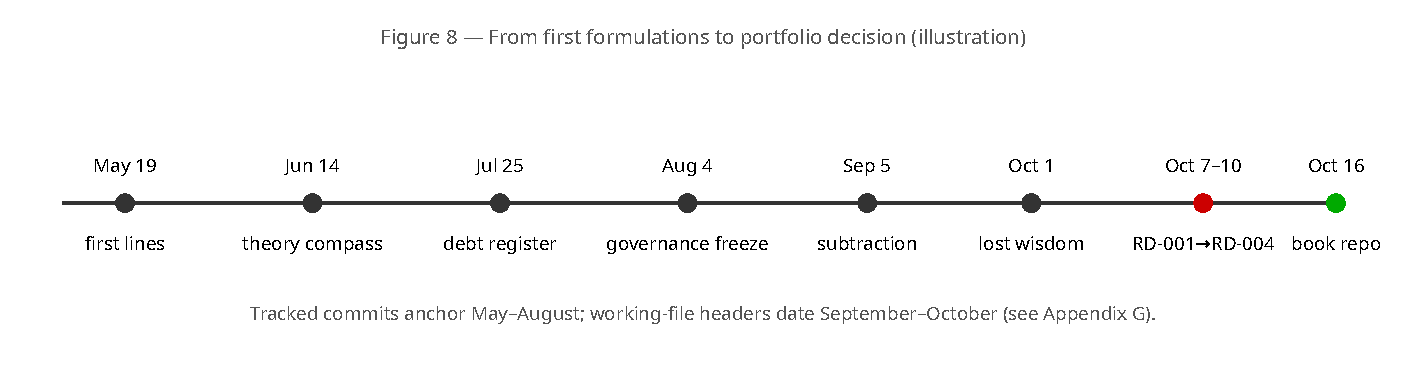
\includegraphics[width=1\linewidth,height=\textheight,keepaspectratio,alt={From first formulations to portfolio decision (illustration)}]{figures/fig8-timeline.pdf}
\caption{From first formulations to portfolio decision (illustration)}
\end{figure}

\newpage

\chapter{Chapter 20. A Philosophical Framework, an Explanatory
Ambition}\label{chapter-20.-a-philosophical-framework-an-explanatory-ambition}

\textbf{The distinction the whole book was building toward:}
SGP-the-metaphysics vs.~SGP-the-explanation
vs.~SGP-the-research-program. Four strategic reviews separated them.
This chapter reports the separation.

\section{RD-001: clarify before
researching}\label{rd-001-clarify-before-researching}

The reorientation disentangled five commitments ---
sentience-as-response, reality-as-sentience,
world-as-experience-content, mathematics-as-possibility, actualization
--- with their dependencies (C2 needs C1; C5 needs C4; C3 needs
C1+C2+C5) and named the two unexamined moves: the \emph{category move}
(property of systems → nature of reality) and the \emph{modal move}
(possibility → actuality). Classification: FOUNDATIONAL CLARIFICATION
REQUIRED BEFORE RESEARCH. The package could not be tested as a unit
because its parts fail differently.

\section{RD-002: coherent, but not
distinctive}\label{rd-002-coherent-but-not-distinctive}

The coherence audit, with provenance tables and seven adversarial
objections (all sustained or partially sustained), found the package
internally consistent --- and mappable onto existing traditions:
Whitehead under the phenomenal reading, structural realism plus James
under the functional reading. The subtraction audit's line: ``nothing
distinctive remains.'' Classification: COHERENT BUT NOT DISTINCTIVE.
Coherence is necessary, not sufficient; the explanatory ambition was
found unearned.

\section{RD-003: familiar concepts, no new
bridge}\label{rd-003-familiar-concepts-no-new-bridge}

The generality chain --- shared perspectives → generality → imbalance →
selection → persistence --- broke on four of six links, each break
requiring time, memory, aggregation, or dynamics the framework does not
contain. The central inference (generality favors actualization) proved
circular or unsupported; reverse causation (persistence \emph{producing}
apparent generality) fit better. Every concept located in prior
literature: Kitcher/Goldman (consensus), Whitehead (prehension),
Tarski/Mac Lane (generality). Classification: FAMILIAR CONCEPTS, NO NEW
EXPLANATORY BRIDGE.

\section{RD-004: the portfolio
decision}\label{rd-004-the-portfolio-decision}

Separating the three layers, the final review judged {[}decisions
reported as decisions, not theorems{]}:

\begin{itemize}
\tightlist
\item
  \textbf{A. The metaphysical commitment} --- COHERENT; NOT FALSIFIED;
  NOT DERIVATIVELY FRUITFUL. Stipulations cannot be false; this one also
  proved barren.
\item
  \textbf{B. The explanatory ambition} --- UNSUPPORTED; SHOULD BE
  SUSPENDED. Structurally foreclosed by informational equivalence:
  physics contains identical information with or without posited
  sentience (I(T;S) = 0).
\item
  \textbf{C. The research program} --- SHOULD CLOSE. Every route tried
  and classified; the one positive output (Paper 3) is independent
  mathematics.
\end{itemize}

Classification: PHILOSOPHICAL FRAMEWORK RETAINED; EXPLANATORY CLAIMS
SUSPENDED. The knowledge graph breaks at persistence→world (15 failed
derivations); observer→experience fails on the combination problem; only
relations→constraints→persistence derives --- all standard mathematics.

\section{The payoff you were promised in the
Prologue}\label{the-payoff-you-were-promised-in-the-prologue}

You can now distinguish, on live examples: a \emph{metaphysical
perspective} (Chapters 1--6: coherent, stipulated, untestable), a
\emph{mathematical discovery} (Chapters 9--10: proved, checked,
philosophy-independent), and a \emph{scientific explanation} (missing
throughout: no constraint, no mechanism, no prediction). Readers who
internalize only one thing from this book should internalize this
three-way split --- it applies far beyond SGP.

\section{Where this chapter leaves
you}\label{where-this-chapter-leaves-you-18}

Framework kept, claims suspended, program closed. Is that the end --- no
future, no hope, no next step? Chapter 21 states exactly what would have
to change for research to honestly resume. The bar is high, and that is
the point.

\newpage

\chapter{Chapter 21. What Would Count as
Progress?}\label{chapter-21.-what-would-count-as-progress}

\textbf{The final discipline:} a closed program must say what would
reopen it --- specifically, falsifiably, and without moving the
goalposts later. RD-004 stated three conditions. This chapter explains
them in plain language and refuses to add a fourth.

\section{Condition 1: a new primitive with independent
motivation}\label{condition-1-a-new-primitive-with-independent-motivation}

Something mathematically real that ordinary relation theory lacks,
needed for reasons \emph{outside} SGP, and carrying physically specific
information the null lacks (breaking I(T;S) = 0). Why this bar: the
equivalence result is structural --- only new information-content
changes it. A relabeled relation does not qualify. Nothing in the
records meets this.

\section{Condition 2: a falsifiable empirical
prediction}\label{condition-2-a-falsifiable-empirical-prediction}

A precise formalization yielding an observable the null does not share,
testable with existing or near-future instruments. Why this bar: the
Compass question is about the world, and only the world can overrule a
null. Engineered predictions with added parameters do not qualify (Exp25
§13 showed why). Nothing in the records meets this.

\section{Condition 3: a non-circular combination
solution}\label{condition-3-a-non-circular-combination-solution}

How micro-experience aggregates to macro-experience, without defining
the conclusion into the premises, yielding new mathematics. Why this
bar: observer→experience is the graph's deepest failure. Stipulated
identities do not qualify. Nothing in the records meets this.

\section{What does NOT qualify (the
anti-list)}\label{what-does-not-qualify-the-anti-list}

No new analogy to a philosophical tradition. No new
sharing/generality/imbalance bridge. No new viability simulation. No new
reading of a stale priority score. And above all: not ``more research
might discover something.'' Hope is not a gate.

\section{The research the book does NOT
propose}\label{the-research-the-book-does-not-propose}

Deliberately, there is no ``Experiment 26'' in these pages. Proposing
one to keep the program alive would violate the portfolio decision this
book reports. The open-questions list (Appendix L) contains only
questions meeting the book's own standard: clear object, noncircular
method, decisive outcome --- and it is short, because most candidates
fail that standard.

\section{Where this chapter leaves
you}\label{where-this-chapter-leaves-you-19}

The horizon is open but guarded: real conditions, real bars, no
promises. The Epilogue returns to where you started --- your own
intuition that the world shouldn't be this intelligible --- and tells
you what the journey was for.

\newpage

\chapter{Epilogue --- The Questions We Carry
Forward}\label{epilogue-the-questions-we-carry-forward}

You began with a feeling every honest person has had: the world is
\emph{too} intelligible. Equations written in solitude predict planets,
particles, condensates. Why?

You have now watched one bold answer attempt the whole journey. Start
from sentience. Build relations, orientation, closure, fibers,
boundaries. Knock on interaction, selection, physics. Document
everything, including the failures. End with a kept philosophy,
suspended claims, and a closed program.

What did the journey buy you? Not a solution. Something better
calibrated: SGP helped \emph{articulate} the questions --- possibility
vs.~actuality, correspondence vs.~mechanism, interpretation
vs.~explanation, stipulation vs.~result. These distinctions are now
yours; they work on any theory, including the ones you love.

And the questions SGP did not answer remain genuinely open: why
mathematics fits experience; why these structures and not others; what,
if anything, actualizes possibilities. No one has answered them. The
Institute's contribution is a map of where one serious attempt stopped
--- with the stopping points surveyed, dated, and labeled, so the next
attempt starts further along.

Do not force triumph. The world is still intelligible, still
unexplained, still waiting. Carry the questions carefully. That was
always the assignment.

\newpage

\begin{figure}
\centering
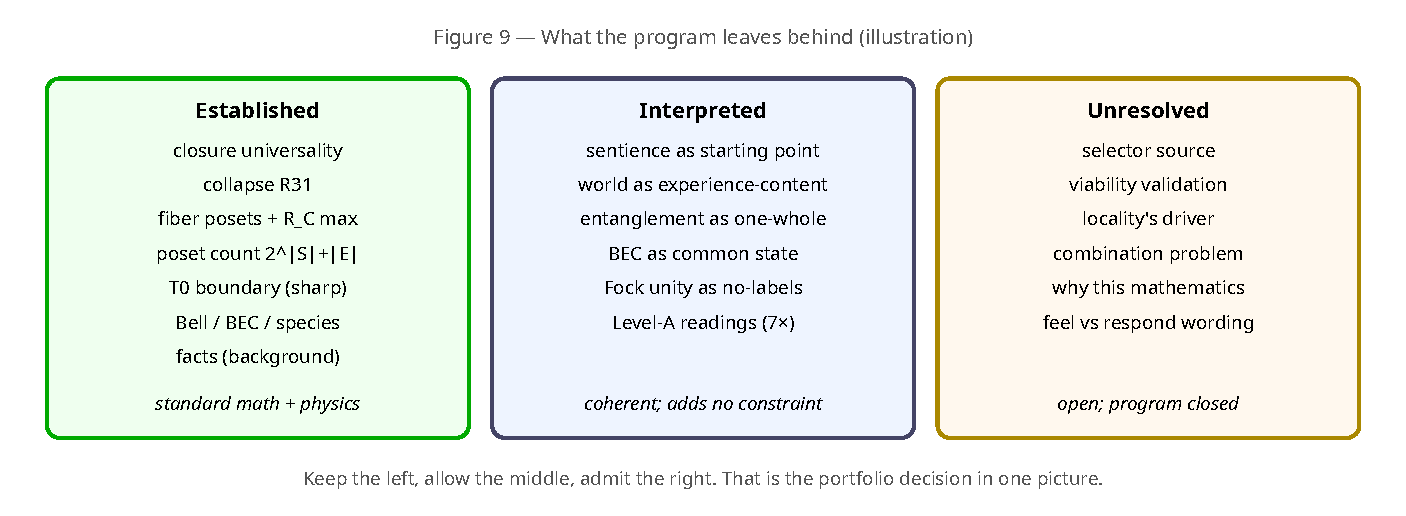
\includegraphics[width=1\linewidth,height=\textheight,keepaspectratio,alt={What the program leaves behind (illustration)}]{figures/fig9-synthesis.pdf}
\caption{What the program leaves behind (illustration)}
\end{figure}

\newpage

\chapter{Appendix A --- The Raw SGP
Vocabulary}\label{appendix-a-the-raw-sgp-vocabulary}

Glossary. Each term: book formulation, original wording, source, date,
revisions. Source: research-map 03-terminology-map.

\begin{itemize}
\tightlist
\item
  \textbf{Sentience (phenomenal).} Book: the capacity to feel, as
  stipulated starting point. Original: ``Sentience (the capacity to
  feel) is the starting point of the research program, not a hypothesis
  to be proved.'' (GOVERNANCE.md:19; frozen 2026-07-26.) Glossary
  repeats (docs/glossary/glossary.md:167).
\item
  \textbf{Sentience (functional).} Book: the ability to respond (to
  another or itself). Original: ``Sentience means the ability to respond
  (a functional definition of sentience, not a phenomenal one).''
  (RD-001:345; 2026-10-07.) Also: ``SENTIENCE = ability to respond;
  response = ordered pair membership'' (Stage1:260).
\item
  \textbf{Sentience (short/unqualified).} ``Sentience is the starting
  point, not a hypothesis to be proved.'' (README.md:13; git
  2026-05-19.)
\item
  \textbf{Sentience (first-person).} ``Treated as self-evident
  first-person reality.'' (RD\_RESEARCH\_COMPASS.md:34; git 2026-06-14.)
  Superseded by governance wording.
\item
  \textbf{Reality.} ``Reality is sentience (identity claim).''
  (RD-001:346.) Earlier: ``REALITY = SENTIENCE''; predecessor
  ``Consciousness (sentience) is ground of being'' (via RD-002:71--78).
\item
  \textbf{Response.} Formal: response(R) ⟺ R≠∅. (Exp24:59--63.) Killed
  readings: verb-like primitive, capacity (Exp22:360).
\item
  \textbf{Experience-content.} ``Physical objects are what sentience
  contains, not what sentience is caused by.'' (RD-001:347.) Earlier:
  ``the `world' as experienced.''
\item
  \textbf{Mathematics (as possibility).} ``About what \emph{could} be,
  not what \emph{is}.'' (RD-001:348.) Least controversial commitment
  (RD-002).
\item
  \textbf{Actualization.} ``Transition from possibility to actuality.''
  (RD-001:349.) Frozen: without selection = standard math
  (differentiator + instability).
\item
  \textbf{Selection.} Distinguished from actualization and
  amplification; source UNRESOLVED (selector audit :83).
\item
  \textbf{Persistence.} ``Remaining stable under perturbation\ldots{}
  what survives repeated interaction.'' (glossary:129--130.) Independent
  property, not part of the primitive (Exp22:176).
\item
  \textbf{Relation.} Set of ordered pairs; specification of which things
  connect to which. (Background.)
\item
  \textbf{Invariant subset / family.} A ⊆ S with R(A) ⊆ A; the family
  Inv(R). (R-program.)
\item
  \textbf{Closure system / operator; fiber; R\_C; essential edge.} See
  Appendix D/I.
\item
  \textbf{C1--C5 (philosophy).} RD-001 package (§2). WARNING: distinct
  from Stage-1 C1--C4 (math grammar: iteration, hierarchy, composition,
  rewriting).
\item
  \textbf{SGP.} This book: sentience-first program. NOTE:
  \texttt{theory/SGP.md:1} defines an unrelated ``Structured Geometry
  Program''; SFI/SFH/SGI identity unresolved (LOST\_WISDOM:249).
\end{itemize}

\newpage

\chapter{Appendix B --- Foundational Statements and
Provenance}\label{appendix-b-foundational-statements-and-provenance}

Source-indexed record of the principal commitments and their formulation
history. See research-map 02-chronology, 03-terminology-map,
07-contradictions.

\section{The five commitments (RD-001:345--351; 2026-10-07, unpublished
working
file)}\label{the-five-commitments-rd-001345351-2026-10-07-unpublished-working-file}

C1 ability-to-respond → C2 reality-is-sentience → C3
world-is-experience-content → C4 mathematics-as-possibility → C5
actualization; dependencies C1→C2, C4→C5, C3 on C1+C2(+C5 per RD-002).
Distinctive moves: category move C1→C2 (:355); modal move C4→C5 (:357).

\section{Provenance per commitment (via RD-002:38--138;
2026-10-08)}\label{provenance-per-commitment-via-rd-00238138-2026-10-08}

\begin{itemize}
\tightlist
\item
  C1: phenomenal (GOVERNANCE:19; glossary:167) vs functional
  (RD-001:345). Discrepancy explicitly recorded (RD-002:32, 59--61,
  503--509). Phenomenal never operationalized; all experiments test
  functional.
\item
  C2: SENTIENCE\_DIFFERENCE\_AUDIT, NULL\_THEORETIC\_LIMIT, SFH O-1
  (cited via RD-002:71--78; primaries not directly re-read --- ``cited
  via'').
\item
  C3: derived term, downstream of sentience + actualization; depends on
  C5 (RD-002:95).
\item
  C4: governance question (:29) + M-formalism (cited via
  RD-002:105--108); ``standard modal-platonist'' (:110).
\item
  C5: frozen sgp\_specific\_structure\_found=false (RD-002:127, citing
  Exp21:445).
\end{itemize}

\section{Compass formulations (drift noted, not
resolved)}\label{compass-formulations-drift-noted-not-resolved}

GOVERNANCE:13--15 (canonical for this book) vs RD\_RESEARCH\_COMPASS:24
vs START\_HERE:10--12 vs GOVERNANCE:271; tension between ``does NOT mean
invent new mathematics'' (:33--38) and ``search for novel structures''
(methodology; RD-001:174).

\section{Date anomalies (marked, not
repaired)}\label{date-anomalies-marked-not-repaired}

GOVERNANCE freeze header 2026-07-26 vs git first-appearance 2026-08-04;
CORE\_ARCHITECTURE header 2025-05-13 vs git 2026-05-19;
\texttt{00\_START\_HERE.md} cited but absent (only
\texttt{START\_HERE.md} exists); RD-001\ldots RD-004 and most audits
untracked (internal dates only); ``capacity'' wording regressing after
Exp22 kill (RD-004:159).

\newpage

\chapter{Appendix C --- The Complete Mathematical
Ladder}\label{appendix-c-the-complete-mathematical-ladder}

Chronological-conceptual list: question, method, result, limitation,
status. Main narrative in Chapters 7--14; theorem index in Appendix D.

\section{Caution on numbering}\label{caution-on-numbering}

Two schemes: V1/V2/T (COMPLETE\_EXPERIMENT\_INVENTORY.md;
\textasciitilde150 exps) vs Exp12--Exp25 (terminal audits). They are NOT
mapped to each other here. Report IDs Exp03--Exp11 not located; Phases
XVIII--XXV as distinct phases not located. Stated as archive gaps.

\section{The ladder}\label{the-ladder}

\begin{enumerate}
\def\labelenumi{\arabic{enumi}.}
\tightlist
\item
  \textbf{Exp12 --- response differentiation.} Orientation forced;
  reciprocity/asymmetry optional; roles = tuple slots. Frozen control.
  (\texttt{SGP\_MINIMAL\_RESPONSE\_MATHEMATICS\_09.md})
\item
  \textbf{Exp13 --- necessity chain.} Difference definitional; weakest =
  bare functional map. Frozen. (Necessity-chain + minimality audits;
  Meta-boundary :84.)
\item
  \textbf{Exp14/15 --- ability vs actuality; self-response minimality.}
  Both coherent (SRMA-3, NULL-0). Frozen grounding.
\item
  \textbf{R29--R31 --- closure minimality + collapse.} Least closure
  system; corrected minimality; three-object unity. Established
  (conditional).
\item
  \textbf{R35 --- reconstruction FALSIFIED.} I\_f ⇏ f (witness pairs
  \textbar S\textbar=3, 4). Negative.
\item
  \textbf{R40 --- universality.} Inv(R) left adjoint; contravariant
  (corrected). Established.
\item
  \textbf{R44--R46/R45 --- R\_C is the unique MAXIMUM} (not minimum).
  Established + correction.
\item
  \textbf{Exp24 --- response vs relation.} 66,067 records; 0 violations;
  0/15; 8/8; verdict. Negative boundary. (Ch. 7.)
\item
  \textbf{Paper 3 --- fiber geometry manuscript.} Thms
  3.1/4.1/5.1/6.1/8.1--8.2; \textbar S\textbar≤4 checks; R64/R65
  internal. Manuscript + finite check; peer review outstanding. (Ch. 9.)
\item
  \textbf{Paper 4 --- poset product + count.} Bijection;
  2\^{}\textbar S\textbar+\textbar E\textbar; \textbar S\textbar≤5
  checks (1,3,19,219,4231). Manuscript + finite check. (Ch. 10.)
\item
  \textbf{R50 --- R46.1 FALSIFIED} (convex sublattices; 7 cex).
  Negative.
\item
  \textbf{R51 --- poset repair.} Finite poset, unique max. Established.
\item
  \textbf{R88/R89 --- T0 essential.} Non-T0 classified; no
  generalization. Established + finite check. (Ch. 11.)
\item
  \textbf{C3 boundary.} Joint determines composition; separate does not
  (\textbar S\textbar≥2). Established; standard math. (Ch. 11.)
\item
  \textbf{Exp19 --- plurality generic.} Zero residue. Negative.
\item
  \textbf{Exp20 --- amplification ≠ selection.} Negative.
\item
  \textbf{Exp21 --- actualization w/o selector = generic math.} Negative
  (for novelty).
\item
  \textbf{Compass I --- NO QUALIFYING QUESTION.} S1/S2/S5 fire. Closed.
  (Ch. 12.)
\item
  \textbf{Selector audit --- UNRESOLVED. Viability --- NOT VALIDATED
  (7×UNRESOLVED).} Open-as-unresolved. (Ch. 12.)
\item
  \textbf{Stage 1 --- C1--C4 exclude nothing.} Negative. (Ch. 13.)
\item
  \textbf{Exp16 --- NO PREDICTIVE BRIDGE.} Negative. (Ch. 13.)
\item
  \textbf{Exp25 --- boxes FAIL; kill 8/8.} Negative. (Ch. 13.)
\item
  \textbf{Road D --- 0/6, all fail D6.} Negative. (Ch. 13.)
\item
  \textbf{RD-001\ldots RD-004 --- clarification /
  coherent-not-distinctive / familiar-concepts / framework-retained.}
  Decisions. (Ch. 20.)
\item
  \textbf{Terminal audits --- P→W FAILED (15 attempts); O→E FAILED;
  I(T;S)=0.} Terminal. (Ch. 20.)
\end{enumerate}

\section{Status key}\label{status-key}

Established (proof) · Finite-check (bounded computation) · Negative
(falsified/boundary) · Unresolved (open, no path) · Manuscript (peer
review outstanding) · Decision (strategic review verdict).

\newpage

\chapter{Appendix D --- Theorem and Proof
Index}\label{appendix-d-theorem-and-proof-index}

Every theorem/lemma/equation discussed, with original location. ``Cited
via'' marks items located through secondary audit tables rather than
direct re-reading; the primary file:line is still given as reported.

\section{Closure program (R-series)}\label{closure-program-r-series}

\begin{itemize}
\tightlist
\item
  R29 (least closure system) --- \texttt{interphase\_a\_notebook.md:733}
  (cited via); ledger \texttt{foundation\_v1.0.md:96,101}.
\item
  R30 correction (closure-system hypothesis required) ---
  \texttt{interphase\_a\_notebook.md:785} (cited via);
  \texttt{foundation\_consolidation\_001.md:55,136}.
\item
  R31 collapse (I\_f = C\_f = cl\_f) ---
  \texttt{interphase\_a\_notebook.md:831,925–929} (cited via);
  \texttt{foundation\_v1.0.md:102}.
\item
  R35 falsification (witnesses f1=\{0↦1,1↦0,2↦1\} vs f2=\{0↦1,1↦0,2↦0\},
  shared I\_f=\{∅,\{0,1\},S\}; second pair sharing \{∅,\{0,2\},S\}) ---
  \texttt{phase033\_r35\_reconstruction\_falsification.md:27–34,42–56,69–84,209–210}.
\item
  R40 universality (Inv ⊣ inclusion; contravariant) ---
  \texttt{interphase\_a\_notebook.md:1139–1155} (cited via);
  \texttt{phase033\_r41\_functor\_audit.md:7,15}.
\item
  R45 (R\_C unique maximum; 13/29 non-minimal, 7 double minima at
  \textbar S\textbar=3) ---
  \texttt{foundation\_consolidation\_001.md:223–235};
  \texttt{foundation\_v1.0.md:62}.
\item
  R50 (R46.1 falsified; 7 cex; ∩-inclusion one-way) ---
  \texttt{phase035\_r50\_foundation\_freeze.md} (cited via);
  corroborated \texttt{paper3\_submission.tex:482–488}.
\item
  R51 (finite poset + unique max; not ∩/∪-closed, not convex, not
  lattice) --- \texttt{foundation\_v1.0.md:108–109};
  \texttt{phase035\_r51\_repair\_campaign.md} (cited via).
\end{itemize}

\section{\texorpdfstring{Paper 3 (submission text
\texttt{papers/paper3\_kernel\_geometry/final/paper3\_submission.tex})}{Paper 3 (submission text papers/paper3\_kernel\_geometry/final/paper3\_submission.tex)}}\label{paper-3-submission-text-paperspaper3_kernel_geometryfinalpaper3_submission.tex}

\begin{itemize}
\tightlist
\item
  Abstract (verified :36--48): Φ: Rel(S)→ClSys(S); image = Alexandrov +
  ∅; unique max R\_C; edge classes; finite poset; conjecture false;
  arbitrary sets/relations.
\item
  Thm 3.1 canonical maximal representative; Thm 4.1 fiber geometry; Thm
  5.1 edge classification (+ Lemma 5.1); Thm 6.1 falsification; Thm
  8.1/8.2 generalization (statements per R64/R65 records; proofs in
  submission text §§3--8).
\item
  Verification scope: \textbar S\textbar≤4 (29 @3, 355 @4; T0-refined
  19/219 --- R88).
\item
  Internal audits: R64 (adversarial verification), R65 (literature
  attack; novelty sentence + folklore caveat).
\end{itemize}

\section{\texorpdfstring{Paper 4
(\texttt{papers/paper4\_fiber\_complexity/paper\_v3.tex} ---
verified)}{Paper 4 (papers/paper4\_fiber\_complexity/paper\_v3.tex --- verified)}}\label{paper-4-paperspaper4_fiber_complexitypaper_v3.tex-verified}

\begin{itemize}
\tightlist
\item
  Abstract (:24): bijection P(S)×P(E); count
  2\^{}\textbar S\textbar+\textbar E\textbar.
\item
  Thm (:46--52): φ(A,E′) = loops(A) ∪ T ∪ E′.
\item
  Proof (:62--79): four paragraphs (verbatim structure in Ch. 10).
\item
  Examples (:83--93): chain-3 → 16; chain-4 → 128; antichain → 2\^{}n; V
  → 8.
\item
  Remark (:95--97): exhaustive check \textbar S\textbar≤5
  (1,3,19,219,4231), zero violations.
\end{itemize}

\section{Boundary results}\label{boundary-results}

\begin{itemize}
\tightlist
\item
  Path Lemma 3.3 (T0 boundary; holds T0, fails non-T0) ---
  \texttt{phase058\_r89\_t0\_boundary.md:21–24,40–44} (cited via).
\item
  Non-T0 fiber = loops × SC-digraphs (10/10) --- \texttt{:92–105} (cited
  via).
\item
  C3 composition boundary (\textbar S\textbar=1 vs ≥2; alignment loss)
  --- \texttt{COMPASS\_I\_BOUNDARY\_RESULT.md:47–54,70–74} (cited via).
\end{itemize}

\section{Finite enumerations (equations reproduced in Ch.
7)}\label{finite-enumerations-equations-reproduced-in-ch.-7}

\begin{itemize}
\tightlist
\item
  Relation census: Σ\_\{n=0..4\} 2\^{}(n²) = 1+2+16+512+65536 = 66,067
  (author-checked arithmetic; reconciles 66,066-nonempty convention).
\item
  Exp24 tallies: 0/66,067 violations; 0/15 required; A=1/B=15/C=0/D=0;
  8/8 formalisms; 10/10 killers; 29/29 engine
  (\texttt{SGP\_RESPONSE\_VS\_RELATION\_AUDIT\_001.md:69,96,272,319,363,390,408,412}
  --- verified).
\item
  Exp25 tallies: 7×A; B=0; C=0; 0/7 selections; 8/8 kills
  (\texttt{SGP\_PHYSICAL\_DISTINCTION\_AUDIT\_001.md:440–475} ---
  verified).
\end{itemize}

\newpage

\chapter{Appendix E --- Negative and Unresolved
Results}\label{appendix-e-negative-and-unresolved-results}

Principal negatives with criterion, evidence, closure. ``Not
established'' ≠ ``disproved'' --- the distinction is kept per row.

\begin{longtable}[]{@{}
  >{\raggedright\arraybackslash}p{(\linewidth - 6\tabcolsep) * \real{0.2500}}
  >{\raggedright\arraybackslash}p{(\linewidth - 6\tabcolsep) * \real{0.2500}}
  >{\raggedright\arraybackslash}p{(\linewidth - 6\tabcolsep) * \real{0.2500}}
  >{\raggedright\arraybackslash}p{(\linewidth - 6\tabcolsep) * \real{0.2500}}@{}}
\toprule\noalign{}
\begin{minipage}[b]{\linewidth}\raggedright
Result
\end{minipage} & \begin{minipage}[b]{\linewidth}\raggedright
Criterion
\end{minipage} & \begin{minipage}[b]{\linewidth}\raggedright
Evidence
\end{minipage} & \begin{minipage}[b]{\linewidth}\raggedright
Reading
\end{minipage} \\
\midrule\noalign{}
\endhead
\bottomrule\noalign{}
\endlastfoot
Response adds nothing over relation & 0/15 required; kill 8/8 & Exp24
(verified) & Not established (distinction); stipulation untouched \\
Reconstruction from consequences & Counterexample pairs & R35 witnesses
& Disproved (as stated) \\
Convex-sublattice fibers & 7 counterexamples & R50 & Disproved; repaired
(R51) \\
Interaction novelty & S1/S2/S5 fire & Compass I P1--P10 & Not
established (question closed) \\
Chirality selects & x0=0 stays 0 & Exp20 & Disproved (selection);
amplification kept \\
Selector exists & Source derivation & Selector audit :83 & UNRESOLVED
(not disproved) \\
Viability validated & 7 kill tests & Viability :40--52 & UNRESOLVED /
not validated \\
C1--C4 constrain physics & Admissibility predicate & Stage1 & Not
established \\
Any physical distinction & Level B/C bar & Exp25 boxes FAIL & Not
established; bridge killed, metaphysics untouched \\
Any Road-D target & D1--D7 gates & Road D 0/6 & Not established \\
Generality → selection & 6-link chain audit & RD-003 (4 broken) & Not
established; concepts familiar \\
Explanatory ambition & Informational equivalence & I(T;S)=0 & Suspended
(structural) \\
P→W derivation & 15 constructions & Terminal audit & Failed attempts
(not impossibility proof) \\
O→E derivation & Combination/constitutive & Terminal audit & Failed
attempts \\
Electron=proton doctrine & Repo-wide search & Negative search (Ch. 17) &
Absent from records (not disproved as physics --- it was never
claimed) \\
Exp03--Exp11 IDs; Phases XVIII--XXV & Archive location & Search negative
& Archive gaps (not findings) \\
\end{longtable}

\newpage

\chapter{Appendix F --- Physics: Established Results vs.~SGP
Interpretations}\label{appendix-f-physics-established-results-vs.-sgp-interpretations}

Columns: phenomenon \textbar{} standard account \textbar{} SGP contact
\textbar{} evidence \textbar{} status.

\begin{longtable}[]{@{}
  >{\raggedright\arraybackslash}p{(\linewidth - 8\tabcolsep) * \real{0.2000}}
  >{\raggedright\arraybackslash}p{(\linewidth - 8\tabcolsep) * \real{0.2000}}
  >{\raggedright\arraybackslash}p{(\linewidth - 8\tabcolsep) * \real{0.2000}}
  >{\raggedright\arraybackslash}p{(\linewidth - 8\tabcolsep) * \real{0.2000}}
  >{\raggedright\arraybackslash}p{(\linewidth - 8\tabcolsep) * \real{0.2000}}@{}}
\toprule\noalign{}
\begin{minipage}[b]{\linewidth}\raggedright
Phenomenon
\end{minipage} & \begin{minipage}[b]{\linewidth}\raggedright
Standard account {[}Established{]}
\end{minipage} & \begin{minipage}[b]{\linewidth}\raggedright
SGP contact
\end{minipage} & \begin{minipage}[b]{\linewidth}\raggedright
Evidence
\end{minipage} & \begin{minipage}[b]{\linewidth}\raggedright
Status
\end{minipage} \\
\midrule\noalign{}
\endhead
\bottomrule\noalign{}
\endlastfoot
Bell correlations & Local hidden variables violate QM statistics;
violations observed to loophole-free level & ``ONE state → two
particles'' reading & Bell 1964; Hensen 2015; Exp25 :139--141 (adds
{[}{]}) & Background + {[}SGP-interpretation{]} \\
No-signaling & Marginal independence (theorem) & None (no SGP claim) &
Textbooks & {[}Established{]} \\
Nonlocality readings & Interpretation-dependent & None examined by
program & Philosophy literature & {[}Established{]} (plurality) \\
BEC & Macroscopic occupation; φ(x) order parameter; Rb-87
\textasciitilde170 nK & ``ONE wavefunction → many particles'' reading &
Anderson/Davis 1995; cases :271--276 (RELATED but DISTINCT) & Background
+ {[}SGP-interpretation{]} \\
Condensate distinctions & Thermal cloud remains; symmetric, not
Bell-like & Institute's own distinction & cases :271--276; textbooks &
{[}Established{]} \\
Species identity & Same-species indistinguishability (Fock
symmetrization) & ``ONE Fock state → N particles'' reading & Textbooks;
cases :43,226 & Background + {[}SGP-interpretation{]} \\
Electron vs proton & Differ: mass, charge, spin class, structure & None
(no record) & PDG; negative search & {[}Established{]}; stronger claim
absent \\
QG emergence & Multiple frameworks coexist & Hoped elimination & 0
eliminations (Exp25; Bridge S1) & {[}SGP-interpretation{]} \\
Holography/QEC & Duality + codes; entanglement→geometry literature &
Controls only & Records decline import & Background \\
Locality origin & Open & Recoverability hope & UNRESOLVED driver &
{[}Unresolved{]} \\
Measurement & Open forks; decoherence partial & Core fork; 0
consciousness shortcuts & Level A only & {[}SGP-interpretation{]} \\
ν-ordering; strong CP; Λ; DM & Open problems & Road-D pools & Gate
failures; I(T;S)=0 & {[}Negative{]} (no bridge) \\
RG/SSB/gauge/arrow & Standard frameworks & Bridge domains & B=0 C=0; 0/7
selections & {[}SGP-interpretation{]} \\
\end{longtable}

Rule used throughout: famous-but-unconnected topics are excluded (see
Ch. 18; research-map 07).

\newpage

\chapter{Appendix G --- Research
Chronology}\label{appendix-g-research-chronology}

Condensed timeline (full: research-map 02-chronology; provenance:
Appendix B).

\begin{itemize}
\tightlist
\item
  \textbf{2026-05-19} --- First formulations committed (README short
  sentience line; CORE\_ARCHITECTURE v2.0 header 2025-05-13 --- gap
  noted).
\item
  \textbf{2026-06-14} --- Theory compass (first-person sentience; ``what
  can persist'').
\item
  \textbf{2026-07-25} --- Debt register: I 27\% / C 54\% / F 79\%
  (origin of the 27\%).
\item
  \textbf{2026-07-26 / 08-04} --- Governance freeze v1.0 (``capacity to
  feel''); glossary; axioms; scope limits (header/git gap noted).
\item
  \textbf{2026-08-16/31} --- Feel-formulations; define-SGP synthesis.
\item
  \textbf{2026-09-05} --- Generative subtraction (``nothing distinctive
  remains''); semantics verdict.
\item
  \textbf{2026-10-01} --- Lost-wisdom compilation (fabrication history;
  provenance caution).
\item
  \textbf{2026-10-07} --- RD-001 (five commitments); Compass I audit (no
  qualifying question).
\item
  \textbf{2026-10-08} --- RD-002 (coherent, not distinctive); Exp24
  (response reduces).
\item
  \textbf{2026-10-09} --- Stage 1 (C1--C4 exclude nothing).
\item
  \textbf{2026-10-10} --- RD-003 (no new bridge); RD-004 (framework
  retained; claims suspended; program closed).
\item
  \textbf{2026-10-16} --- SGP-Book repository created (this book's
  destination).
\item
  \textbf{Manuscript track} --- Paper 3 RC1 + R64/R65 + R88/R89
  corrections; Paper 4 v3 (abstract correction; \textbar S\textbar≤5
  checks).
\end{itemize}

Uncertain dates marked in research-map 02; internal headers are
self-reported, not independently corroborated.

\newpage

\chapter{Appendix H --- Research Status and Closure
Register}\label{appendix-h-research-status-and-closure-register}

Why each branch closed; what new evidence would justify reconsideration
(mirrors RD-004 §10: only the three stated conditions).

\begin{longtable}[]{@{}
  >{\raggedright\arraybackslash}p{(\linewidth - 4\tabcolsep) * \real{0.3333}}
  >{\raggedright\arraybackslash}p{(\linewidth - 4\tabcolsep) * \real{0.3333}}
  >{\raggedright\arraybackslash}p{(\linewidth - 4\tabcolsep) * \real{0.3333}}@{}}
\toprule\noalign{}
\begin{minipage}[b]{\linewidth}\raggedright
Branch
\end{minipage} & \begin{minipage}[b]{\linewidth}\raggedright
Why closed
\end{minipage} & \begin{minipage}[b]{\linewidth}\raggedright
Reconsider iff
\end{minipage} \\
\midrule\noalign{}
\endhead
\bottomrule\noalign{}
\endlastfoot
Response formalism & 0/66,067; 0/15; 8/8 (Exp24) & New primitive with
independent motivation (Cond. 1) \\
Orientation program & Standard relation theory & --- (background, not a
claim) \\
Reconstruction & Counterexamples (R35) & New construction outside stated
hypotheses \\
Convex fibers & Counterexamples (R50) & --- (repaired by R51) \\
Interaction mathematics & No qualifying question (Compass I) & Cond.
1 \\
Selection/viability & UNRESOLVED source; unvalidated dynamics & Cond. 1
or genuine mechanism (not relabeling) \\
Generality bridge & 4/6 links broken (RD-003) & Cond. 1 \\
C1--C4 physics grammar & Excludes nothing (Stage 1) & Cond. 2
(prediction) \\
Empirical bridge & Boxes FAIL; kill 8/8 (Exp25) & Cond. 2 \\
Residual anomalies & 0/6; D6 failures (Road D) & Cond. 2 \\
Explanatory ambition & I(T;S)=0 (structural) & Cond. 1 or 2 \\
Combination problem & Failed attempts (terminal) & Cond. 3 \\
Metaphysical commitment & --- (never closed; retained as coherent
stipulation) & N/A \\
Paper 3 / Paper 4 & --- (not closed; manuscripts; peer review
outstanding) & Publication process \\
\end{longtable}

RD-001\ldots RD-004 decisions: clarification required /
coherent-not-distinctive / familiar-concepts /
framework-retained-claims-suspended (Ch. 20). Archive gaps: Exp03--Exp11
IDs; Phases XVIII--XXV (stated, not hidden). Retraction pattern note:
headlines vs deep-tree corrections (LOST\_WISDOM) --- the register rule:
no headline without a source row.

\newpage

\chapter{Appendix I --- Mathematical and Scientific
Glossary}\label{appendix-i-mathematical-and-scientific-glossary}

Plain-language definitions for the general reader. (Foundational SGP
vocabulary: Appendix A.)

\begin{itemize}
\tightlist
\item
  \textbf{Relation.} A list of connections between dots: which pairs (x,
  y) are linked, including self-links (x, x).
\item
  \textbf{Ordered pair / orientation.} (x, y) ≠ (y, x): arrows have
  direction. Reciprocity and asymmetry are extra, optional properties.
\item
  \textbf{Isomorphism.} A renaming of dots preserving all connections;
  isomorphic structures are ``the same up to labels.''
\item
  \textbf{Invariant subset.} A collection no arrow leaves: R(A) ⊆ A.
\item
  \textbf{Closure system.} A family of subsets containing S and closed
  under intersection --- the shape of ``consequence structures.''
\item
  \textbf{Closure operator.} The rule sending each set to the smallest
  closed set containing it (everything it implies).
\item
  \textbf{Fiber.} All relations sharing one consequence-structure: F\_C
  = \{R : Inv(R) = C\}.
\item
  \textbf{Canonical / maximal representative (R\_C).} The largest wiring
  with given consequences; unique top of the fiber.
\item
  \textbf{Essential vs.~conditionally removable edge.} Must-stay
  vs.~may-go wires of R\_C.
\item
  \textbf{Partial order.} A ranking with possible incomparabilities
  (prerequisites).
\item
  \textbf{Lower set.} Downward-closed collection (with prerequisites
  included).
\item
  \textbf{Covering pair.} A direct prerequisite link with nothing
  between.
\item
  \textbf{Transitive reduction (T).} The skeleton of covering pairs.
\item
  \textbf{Alexandrov topology.} Consequence-structures closed under
  arbitrary intersection (finite case: no restriction).
\item
  \textbf{T0.} The structure tells every pair of dots apart (no
  duplicates).
\item
  \textbf{Composition.} Chaining relations end to end (R followed by S).
\item
  \textbf{Quantum state.} The vector encoding a system's measurable
  tendencies.
\item
  \textbf{Entanglement.} Joint state that doesn't factor into parts;
  Bell violations; no-signaling respected.
\item
  \textbf{Partial trace / reduced state.} The shadow of the whole
  visible from one part.
\item
  \textbf{Boson / fermion.} Shareable-state vs.~exclusive-state particle
  classes (Pauli exclusion for fermions).
\item
  \textbf{Condensation (BEC).} Macroscopic occupation of one quantum
  state; order parameter φ(x).
\item
  \textbf{Identical particles.} Same-species indistinguishability via
  symmetrized states; occupation numbers; Fock space. Cross-species
  identity is NOT implied.
\end{itemize}

\newpage

\chapter{Appendix J --- Annotated
Bibliography}\label{appendix-j-annotated-bibliography}

External sources: see references/bibliography.md (full annotations: what
each supports / does not support). Institute primary sources: see
research-map 01-source-inventory and Appendix D (theorems) / Appendix H
(closure register).

Reading rule (from references/source-notes.md): Institute citations are
\texttt{path:line} in the source working tree. ``Unpublished working
file'' = internal date, no git history, not a publication. ``Cited via''
= located through secondary audit tables. Manuscripts = LaTeX sources
with stated scope + internal audits; peer review outstanding. DOIs for
Bell 1964, Anderson 1995, Davis 1995, Hensen 2015 verified live;
remaining external refs are canonical/textbook-stable.

\newpage

\chapter{Appendix K --- Reproducibility and Computational
Record}\label{appendix-k-reproducibility-and-computational-record}

Only materials that can be safely and legally described. No datasets or
engines are copied into this book; paths let a reader with repository
access re-run them. Nothing here is claimed reproducible beyond what the
records state.

\begin{longtable}[]{@{}
  >{\raggedright\arraybackslash}p{(\linewidth - 6\tabcolsep) * \real{0.2500}}
  >{\raggedright\arraybackslash}p{(\linewidth - 6\tabcolsep) * \real{0.2500}}
  >{\raggedright\arraybackslash}p{(\linewidth - 6\tabcolsep) * \real{0.2500}}
  >{\raggedright\arraybackslash}p{(\linewidth - 6\tabcolsep) * \real{0.2500}}@{}}
\toprule\noalign{}
\begin{minipage}[b]{\linewidth}\raggedright
Computation
\end{minipage} & \begin{minipage}[b]{\linewidth}\raggedright
Engine → output (source repo)
\end{minipage} & \begin{minipage}[b]{\linewidth}\raggedright
Reported result
\end{minipage} & \begin{minipage}[b]{\linewidth}\raggedright
Reproducibility note
\end{minipage} \\
\midrule\noalign{}
\endhead
\bottomrule\noalign{}
\endlastfoot
Exp24 census &
\texttt{experiments/interaction\_rule\_space/exp24\_response\_vs\_relation\_engine.py}
→ \texttt{exp24\_response\_vs\_relation\_result.json} & 29/29; 0/66,067
& Deterministic (seed 24; reruns byte-identical modulo runtime) \\
Exp25 audits & parts 01--28 in
\texttt{SGP\_PHYSICAL\_DISTINCTION\_AUDIT\_001.md} & 7×A; boxes FAIL;
kill 8/8 & Finite declared inventories; exact counts \\
C2 hierarchy & \texttt{c2\_hierarchy\_engine.py} →
\texttt{c2\_hierarchy\_engine\_result.\{txt,json\}} & 66,066 relations;
9 classes; 54 strict; 29 incomparable; 10 covers & Authoritative run
DONE in 131.0s \\
Paper 3 checks & \texttt{papers/paper3\_kernel\_geometry/computations/}
& & S \\
Paper 4 checks & remark in \texttt{paper\_v3.tex:95–97} & & S \\
R88/R89 & brute force n=3,4 T0 vs non-T0 & 10 non-T0 violations; 0/219
T0 & Scope stated in phase records \\
Frozen controls & md5 baselines in Exp24 §1 (26 files) & Unchanged after
write & Integrity mechanism, not science \\
\end{longtable}

Software environments are not pinned in the records consulted; reruns
may differ cosmetically (e.g.~runtime fields). The book's mathematical
claims rest on proofs and stated scopes, not on re-execution.

\newpage

\chapter{Appendix L --- Open Questions}\label{appendix-l-open-questions}

Only questions with a clear object, a noncircular method, and a decisive
outcome. Closed branches are NOT reworded into tasks (see Appendix H).

\begin{enumerate}
\def\labelenumi{\arabic{enumi}.}
\tightlist
\item
  \textbf{Peer review of the fiber manuscripts.} Object: Paper 3 / Paper
  4 claims. Method: journal refereeing. Decisive: publish / revise /
  refute. (Independent of SGP metaphysics.)
\item
  \textbf{The three resume conditions (RD-004 §10).} (a) New primitive
  with independent motivation breaking I(T;S)=0. (b) Falsifiable
  empirical prediction the null lacks. (c) Non-circular combination
  solution yielding new math. Each has a clear object and verdict; none
  is currently met.
\item
  \textbf{Archive completion.} Object: Exp03--Exp11 IDs; Phases
  XVIII--XXV records. Method: provenance search. Decisive: found
  (integrate) or confirmed-absent (close gap). Historical, not
  scientific.
\item
  \textbf{Terminology adjudication.} Object: phenomenal vs functional
  sentience. Method: stipulative decision by any successor program (not
  an experiment --- stipulations aren't testable). Decisive: one wording
  adopted consistently.
\item
  \textbf{The Compass question itself.} ``Why does mathematics describe
  stable experience?'' --- open to philosophy and science generally,
  with no SGP privilege. Listed so no one mistakes closure of the
  program for closure of the question.
\end{enumerate}

Everything else in the records is closed (Appendix H) or background
(Appendix F).

\newpage

\chapter{Appendix M --- Claim Classification and Evidence
Key}\label{appendix-m-claim-classification-and-evidence-key}

Labels used consistently throughout the book (shown in brackets after
claims):

\begin{itemize}
\tightlist
\item
  \textbf{{[}Established{]}} --- Settled science or textbook mathematics
  (e.g.~Bell violations; symmetrization; 2\^{}(n²) census arithmetic).
\item
  \textbf{{[}Math-verified{]}} --- Proved in the records (theorems,
  audit reasoning). Manuscript proofs are marked ``-as-manuscript'' with
  peer review outstanding.
\item
  \textbf{{[}Finite-check{]}} --- Exhaustively computed within a stated
  finite scope (\textbar X\textbar≤4; \textbar S\textbar≤5), not a
  general proof.
\item
  \textbf{{[}SGP-commitment{]}} --- Foundational stipulation or
  Institute position (C1--C5; governance question). Not testable; can be
  coherent or incoherent.
\item
  \textbf{{[}SGP-interpretation{]}} --- The Institute's reading of
  standard material (Level A). Allowed; adds no constraint.
\item
  \textbf{{[}SGP-hypothesis{]}} --- Speculative proposal under
  investigation (e.g.~ONE-EQUATION pattern before downgrade). Testable
  in principle.
\item
  \textbf{{[}Author-inference{]}} --- This book's own synthesis,
  arithmetic, or framing. Checkable; not attributed to the records.
\item
  \textbf{{[}Negative{]}} --- Falsified, bounded, or closed-against
  (R35; Exp24/25 verdicts; Road D). Includes ``absent from records''
  search results.
\item
  \textbf{{[}Unresolved{]}} --- Open with no current path (selector
  source; viability; locality driver) or open-with-path (Appendix L).
\end{itemize}

Combinations occur (e.g.~``{[}Established{]} + {[}Negative{]}'' where
the records confirm standard physics and close the SGP add-on). The
label travels with the claim in every chapter.

\backmatter
\end{document}
